%%%%%%%%%%%%%%%%%%%%%%%%%%%%%%%%%%%%%%%%%%%%%%%%%%%%%%%%%%%%%%%%%%%%%%%%%%%%%%%%
%  Zawartość: Główny plik szablonu pracy dyplomowej (magisterskiej/inżynierskiej).
%  Opracował: Tomasz Kubik <tomasz.kubik@pwr.edu.pl>
%  Data: 28 grudnia 2022
%  Wersja: 0.8
%  Wymagania: kompilator pdflatex
%%%%%%%%%%%%%%%%%%%%%%%%%%%%%%%%%%%%%%%%%%%%%%%%%%%%%%%%%%%%%%%%%%%%%%%%%%%%%%%
\documentclass[a4paper,onecolumn,oneside,12pt,extrafontsizes]{memoir}
\usepackage[giveninits=true]{biblatex}
\addbibresource{dokumentacja.bib}
%  W celu przygotowania wydruku do archiwum można:
%  a) przygotować pdf, w którym dwie strony zostaną wstawione na jedną fizyczną stronę i taki dokument wydrukować dwustronnie (podejście zalecane)
%
%   Taki dokument można przygotować poprzez
%   - wydruk z Adobe Acrobat Reader z opcją "Wiele" - sekcja "Rozmiar i obsługa stron"
%   - wykorzystanie narzędzi psutils
%
%      Windows (zakładając, że w dystrybucji MiKTeX jest pakiet miktex-psutils-bin-x64-2.9):
%        "c:\Program Files\MiKTeX 2.9\miktex\bin\x64\pdf2ps.exe" Dyplom.pdf Dyplom.ps
%        "c:\Program Files\MiKTeX 2.9\miktex\bin\x64\psnup.exe" -2 Dyplom.ps Dyplom2.ps
%        "c:\Program Files\MiKTeX 2.9\miktex\bin\x64\ps2pdf.exe" Dyplom2.ps Dyplom2.pdf
%        Del Dyplom2.ps Dyplom.ps
%
%     Linux:
%        pdf2ps Dyplom.pdf - | psnup -2 | ps2pdf - Dyplom2.pdf
%
%  b) przekomplilować dokument zmniejszając czcionkę (podejście niezalecane, bo zmienia formatowanie dokumentu)
%
%    Do tego wystarczy posłużyć się poniższymi komendami (zamiast documentclass z pierwszej linijki):
%   \documentclass[a4paper,onecolumn,twoside,10pt]{memoir}
%   \renewcommand{\normalsize}{\fontsize{8pt}{10pt}\selectfont}

%\usepackage[cp1250]{inputenc} % Proszę zostawić, jeśli kodowanie edytowanych plików to cp1250
\usepackage[utf8]{inputenc} % Proszę użyć zamiast powyższego, jeśli kodowanie edytowanych plików to UTF8
\usepackage[T1]{fontenc}
\usepackage{color}
\usepackage[english,polish]{babel} % Tutaj ważna jest kolejność atrybutów (dla pracy po polsku polish powinno być na końcu)
%\DisemulatePackage{setspace}
\usepackage{setspace}
\usepackage{color,calc}
%\usepackage{soul} % pakiet z komendami do podkreślania, przekreślania, podświetlania tekstu (raczej niepotrzebny)
\usepackage{ebgaramond} % pakiet z czcionkami garamond, potrzebny tylko do strony tytułowej, musi wystąpić przed pakietem tgtermes

%% Aby uzyskać polskie literki w pdfie (a nie zlepki) korzystamy z pakietu czcionek tgterms.
%% W pakiecie tym są zdefiniowane klony czcionek Times o kształtach: normalny, pogrubiony, italic, italic pogrubiony.
%% W pakiecie tym brakuje czcionki o kształcie: slanted (podobny do italic).
%% Jeśli w dokumencie gdzieś zostanie zastosowana czcionka slanted (np. po użyciu komendy \textsl{}), to
%% latex dokona podstawienia na czcionkę standardową i zgłosi to w ostrzeżeniu (warningu).
%% Ponadto tgtermes to czcionka do tekstu. Wszelkie matematyczne wzory będą sformatowane domyślną czcionką do wzorów.
%% Jeśli wzory mają być sformatowane z wykorzystaniem innych czcionek, trzeba to jawnie zadeklarować.

%% Po zainstalowaniu pakietu tgtermes może będzie trzeba zauktualizować informacje
%% o dostępnych fontach oraz mapy. Można to zrobić z konsoli (jako administrator)
%% initexmf --admin --update-fndb
%% initexmf --admin --mkmaps

\usepackage{tgtermes}
\renewcommand*\ttdefault{txtt}


%%%%%%%%%%%%%%%%%%%%%%%%%%%%%%%%%%%%%%%%%%%%%%%%%%%%%%%%%%%%%%%%%%%%%%%%%%%%%%%%
%% Ustawienia odpowiedzialne za sposób łamania dokumentu
%% i ułożenie elementów pływających
%%%%%%%%%%%%%%%%%%%%%%%%%%%%%%%%%%%%%%%%%%%%%%%%%%%%%%%%%%%%%%%%%%%%%%%%%%%%%%%%
\hyphenpenalty=10000		% nie dziel wyrazów zbyt często
\clubpenalty=10000      % kara za sierotki
\widowpenalty=10000     % nie pozostawiaj wdów
\brokenpenalty=10000		% nie dziel wyrazów między stronami - trzeba było wyłączyć, bo nie łamały się linie w lstlisting
\exhyphenpenalty=999999		% nie dziel słów z myślnikiem - trzeba było wyłączyć, bo nie łamały się linie w lstlisting
\righthyphenmin=3			  % dziel minimum 3 litery

%\tolerance=4500
%\pretolerance=250
%\hfuzz=1.5pt
%\hbadness=1450

\renewcommand{\topfraction}{0.95}
\renewcommand{\bottomfraction}{0.95}
\renewcommand{\textfraction}{0.05}
\renewcommand{\floatpagefraction}{0.35}

%%%%%%%%%%%%%%%%%%%%%%%%%%%%%%%%%%%%%%%%%%%%%%%%%%%%%%%%%%%%%%%%%%%%%%%%%%%%%%%%
%%  Ustawienia rozmiarów: tekstu, nagłówka i stopki, marginesów
%%  dla dokumentów klasy memoir
%%%%%%%%%%%%%%%%%%%%%%%%%%%%%%%%%%%%%%%%%%%%%%%%%%%%%%%%%%%%%%%%%%%%%%%%%%%%%%%%
\setlength{\headsep}{10pt}
\setlength{\headheight}{13.6pt} % wartość baselineskip dla czcionki 11pt tj. \small wynosi 13.6pt
\setlength{\footskip}{\headsep+\headheight}
\setlength{\uppermargin}{\headheight+\headsep+1cm}
\setlength{\textheight}{\paperheight-\uppermargin-\footskip-1.5cm}
\setlength{\textwidth}{\paperwidth-5cm}
\setlength{\spinemargin}{2.5cm}
\setlength{\foremargin}{2.5cm}
\setlength{\marginparsep}{2mm}
\setlength{\marginparwidth}{2.3mm}
%\settrimmedsize{297mm}{210mm}{*}
%\settrims{0mm}{0mm}
\checkandfixthelayout[fixed] % konieczne, aby się dobrze wszystko poustawiało
%%%%%%%%%%%%%%%%%%%%%%%%%%%%%%%%%%%%%%%%%%%%%%%%%%%%%%%%%%%%%%%%%%%%%%%%%%%%%%%%
%%  Ustawienia odległości linii, wcięć, odstępów
%%%%%%%%%%%%%%%%%%%%%%%%%%%%%%%%%%%%%%%%%%%%%%%%%%%%%%%%%%%%%%%%%%%%%%%%%%%%%%%%
\linespread{1}
%\linespread{1.241}
\setlength{\parindent}{14.5pt}


\usepackage{multicol} % pakiet umożliwiający stworzenie wielokolumnowego tekstu
%%%%%%%%%%%%%%%%%%%%%%%%%%%%%%%%%%%%%%%%%%%%%%%%%%%%%%%%%%%%%%%%%%%%%%%%%%%%%%%%
%% Pakiety do formatowania tabel
%%%%%%%%%%%%%%%%%%%%%%%%%%%%%%%%%%%%%%%%%%%%%%%%%%%%%%%%%%%%%%%%%%%%%%%%%%%%%%%%
\usepackage{tabularx}
% Proszę używać tylko tabularx. Innych pakietów proszę nie stosować !!!
% Dokument na pewno da się zredagować bez ich użycia.
%\usepackage{longtable}
%\usepackage{ltxtable}
%\usepackage{tabulary}

%%%%%%%%%%%%%%%%%%%%%%%%%%%%%%%%%%%%%%%%%%%%%%%%%%%%%%%%%%%%%%%%%%%%%%%%%%%%%%%%
%% Pakiet do wstawiania fragmentów kodu
%%%%%%%%%%%%%%%%%%%%%%%%%%%%%%%%%%%%%%%%%%%%%%%%%%%%%%%%%%%%%%%%%%%%%%%%%%%%%%%%
\usepackage{listings}
\usepackage{xpatch}
\makeatletter
\xpatchcmd\l@lstlisting{1.5em}{0em}{}{}
\makeatother
% Pakiet dostarcza otoczenia lstlisting. Jest ono wysoce konfigurowalne.
% Konfigurować można indywidualnie każdy z listingów lub globalnie, w poleceniu \lstset{}.

% Zalecane jest, by kod źródłowy był wyprowadzany z użyciem czcionki maszynowej \ttfamily
% Ponieważ kod źródłowy, nawet po obcięciu do interesujących fragmentów, bywa obszerny, należy zmniejszyć czcionkę.
% Zalecane jest \small (dla krótkich fragmentów) oraz \footnotesize (dla dłuższych fragmentów).

% Ponadto podczas konfiguracji można zadeklarować sposób numerowania linii. Numerowanie linii zalecane jest jednak
% tylko w przypadkach, gdy w redagowanym tekście znajdują się jakieś odwołania do konkretnych linii.
% Jeśli takich odwołań nie ma, numerowanie linii jest zbędne. Proszę wtedy go nie stosować.
% Przy włączaniu numerowania linii należy zwrócić uwagę na to, gdzie pojawią się te numery.
% Bez zmiany dodatkowych parametrów pojawiają się one na marginesie strony (co jest niepożądane).

\lstset{
	basicstyle=\small\ttfamily, % lub basicstyle=\footnotesize\ttfamily
%%columns=fullflexible,
%%showstringspaces=false,
%%showspaces=false,
	breaklines=true,
	postbreak=\mbox{\textcolor{red}{$\hookrightarrow$}\space},
%%numbers=left,  % ta i poniższe linie dotyczą ustawienia numerowania i sposobu jego wyprowadzania
%%firstnumber=1,
%%numberfirstline=true,
%%xleftmargin=17pt,
%%framexleftmargin=17pt,
%%framexrightmargin=5pt,
%%framexbottommargin=4pt,
	belowskip=.5\baselineskip,
	literate={\_}{{\_\allowbreak}}1 % ta deklaracja przydaje się, jeśli na listingu mają być łamane nazwy zawierające podkreślniki
}

% Jeśli edytowany plik nie jest w kodowaniu cp1250, to jest problem z polskimi znakami występującymi we wstawianym kodzie.
% Dlatego podczas pracy na plikach w kodowaniu UTF8 trzeba zadeklarować mapowanie jak niżej (wystarczy odmarkować).
% Niestety, jak się zastosuje to mapowanie mogą pojawić się problemy z podświetlaniem składni (patrz dalej).
%%\lstset{literate=%-
%%{ą}{{\k{a}}}1 {ć}{{\'c}}1 {ę}{{\k{e}}}1 {ł}{{\l{}}}1 {ń}{{\'n}}1 {ó}{{\'o}}1 {ś}{{\'s}}1 {ż}{{\.z}}1 {ź}{{\'z}}1 {Ą}{{\k{A}}}1 {Ć}{{\'C}}1 {Ę}{{\k{E}}}1 {Ł}{{\L{}}}1 {Ń}{{\'N}}1 {Ó}{{\'O}}1 {Ś}{{\'S}}1 {Ż}{{\.Z}}1 {Ź}{{\'Z}}1
%%{Ö}{{\"O}}1
%%{Ä}{{\"A}}1
%%{Ü}{{\"U}}1
%%{ß}{{\ss}}1
%%{ü}{{\"u}}1
%%{ä}{{\"a}}1
%%{ö}{{\"o}}1
%%{~}{{\textasciitilde}}1
%%{—}{{{\textemdash} }}1
%%}%{\ \ }{{\ }}1}


%% lstlisting pozwala na ostylowania podświetlania składni wybranych języków.
%% Działa to na zasadzie zdefiniowania słów kluczowych oraz sposobu ich wyświetlania.
%% Ponieważ jest to prosty mechanizm, czasem trudno osiągnąć takie efekty, jakie dają narzędzia IDE.
%% Jednak w większości przypadku osiągane rezutlaty są zadowalające.


%% lstlisting obsługuje domyślnie kilka najpopularniejszych języków.
%%\lstloadlanguages{% Check Dokumentation for further languages ...
%%C,
%%C++,
%%csh,
%%Java
%%}
%% Inne języki muszą być dodefiniowane. Poniżej podano przykłady definicji języków i styli.

\definecolor{lightgray}{rgb}{.9,.9,.9}
\definecolor{darkgray}{rgb}{.4,.4,.4}
\definecolor{purple}{rgb}{0.65, 0.12, 0.82}
\definecolor{javared}{rgb}{0.6,0,0} % for strings
\definecolor{javagreen}{rgb}{0.25,0.5,0.35} % comments
\definecolor{javapurple}{rgb}{0.5,0,0.35} % keywords
\definecolor{javadocblue}{rgb}{0.25,0.35,0.75} % javadoc

\lstdefinelanguage{JavaScript}{
	keywords={typeof, new, true, false, catch, function, return, null, catch, switch, var, if, in, while, do, else, case, break},
	keywordstyle=\color{blue}\bfseries,
	ndkeywords={class, export, boolean, throw, implements, import, this},
	ndkeywordstyle=\color{darkgray}\bfseries,
	identifierstyle=\color{black},
	sensitive=false,
	comment=[l]{//},
	morecomment=[s]{/*}{*/},
	commentstyle=\color{purple}\ttfamily,
	stringstyle=\color{red}\ttfamily,
	morestring=[b]',
	morestring=[b]"
}
\lstdefinestyle{JavaScriptStyle}{
	language=JavaScript,
	commentstyle=\color{javagreen}, % niestety, jeśli w linii komentarza pojawią się słowa kluczowe, to zostaną pokolorowane
	backgroundcolor=,%\color{lightgray}, % można ustwić kolor tła, ale jest to niezalecane
	extendedchars=true,
	basicstyle=\footnotesize\ttfamily,
	showstringspaces=false,
	showspaces=false,
	numbers=none,%left,
	numberstyle=\footnotesize,
	numbersep=9pt,
	tabsize=2,
	breaklines=true,
	showtabs=false,
	captionpos=t
}

\lstdefinestyle{JavaStyle}{
	basicstyle=\footnotesize\ttfamily,
	keywordstyle=\color{javapurple}\bfseries,
	stringstyle=\color{javared},
	commentstyle=\color{javagreen},
	morecomment=[s][\color{javadocblue}]{/**}{*/},
	numbers=none,%left,
	numberstyle=\tiny\color{black},
	stepnumber=2,
	numbersep=10pt,
	tabsize=4,
	showspaces=false,
	showstringspaces=false,
	captionpos=t
}

\definecolor{pblue}{rgb}{0.13,0.13,1}
\definecolor{pgreen}{rgb}{0,0.5,0}
\definecolor{pred}{rgb}{0.9,0,0}
\definecolor{pgrey}{rgb}{0.46,0.45,0.48}
\definecolor{dark-grey}{rgb}{0.4,0.4,0.4}
% styl json
\newcommand\JSONnumbervaluestyle{\color{blue}}
\newcommand\JSONstringvaluestyle{\color{red}}

\newif\ifcolonfoundonthisline

\makeatletter

\lstdefinestyle{json-style}
{
	showstringspaces    = false,
	keywords            = {false,true},
	alsoletter          = 0123456789.,
	morestring          = [s]{"}{"},
	stringstyle         = \ifcolonfoundonthisline\JSONstringvaluestyle\fi,
	MoreSelectCharTable =%
	\lst@DefSaveDef{`:}\colon@json{\processColon@json},
	basicstyle          = \footnotesize\ttfamily,
	keywordstyle        = \ttfamily\bfseries,
	numbers				= left, % zakomentować, jeśli numeracja linii jest niepotrzebna
	numberstyle={\footnotesize\ttfamily\color{dark-grey}},
	xleftmargin			= 2em % zakomentować, jeśli numeracja linii jest niepotrzebna
}

\newcommand\processColon@json{%
	\colon@json%
	\ifnum\lst@mode=\lst@Pmode%
	\global\colonfoundonthislinetrue%
	\fi
}

\lst@AddToHook{Output}{%
	\ifcolonfoundonthisline%
	\ifnum\lst@mode=\lst@Pmode%
	\def\lst@thestyle{\JSONnumbervaluestyle}%
	\fi
	\fi
	\lsthk@DetectKeywords%
}

\lst@AddToHook{EOL}%
{\global\colonfoundonthislinefalse}

\makeatother

%%\definecolor{red}{rgb}{0.6,0,0} % for strings
%%\definecolor{blue}{rgb}{0,0,0.6}
%%\definecolor{green}{rgb}{0,0.8,0}
%%\definecolor{cyan}{rgb}{0.0,0.6,0.6}
%%
%%\lstdefinestyle{sqlstyle}{
%%language=SQL,
%%basicstyle=\footnotesize\ttfamily,
%%numbers=left,
%%numberstyle=\tiny,
%%numbersep=5pt,
%%tabsize=2,
%%extendedchars=true,
%%breaklines=true,
%%showspaces=false,
%%showtabs=true,
%%xleftmargin=17pt,
%%framexleftmargin=17pt,
%%framexrightmargin=5pt,
%%framexbottommargin=4pt,
%%keywordstyle=\color{blue},
%%commentstyle=\color{green},
%%stringstyle=\color{red},
%%}
%%
%%\lstdefinestyle{sharpcstyle}{
%%language=[Sharp]C,
%%basicstyle=\footnotesize\ttfamily,
%%numbers=left,
%%numberstyle=\tiny,
%%numbersep=5pt,
%%tabsize=2,
%%extendedchars=true,
%%breaklines=true,
%%showspaces=false,
%%showtabs=true,
%%xleftmargin=17pt,
%%framexleftmargin=17pt,
%%framexrightmargin=5pt,
%%framexbottommargin=4pt,
%%morecomment=[l]{//}, %use comment-line-style!
%%morecomment=[s]{/*}{*/}, %for multiline comments
%%showstringspaces=false,
%%morekeywords={  abstract, event, new, struct,
%%as, explicit, null, switch,
%%base, extern, object, this,
%%bool, false, operator, throw,
%%break, finally, out, true,
%%byte, fixed, override, try,
%%case, float, params, typeof,
%%catch, for, private, uint,
%%char, foreach, protected, ulong,
%%checked, goto, public, unchecked,
%%class, if, readonly, unsafe,
%%const, implicit, ref, ushort,
%%continue, in, return, using,
%%decimal, int, sbyte, virtual,
%%default, interface, sealed, volatile,
%%delegate, internal, short, void,
%%do, is, sizeof, while,
%%double, lock, stackalloc,
%%else, long, static,
%%enum, namespace, string},
%%keywordstyle=\color{cyan},
%%identifierstyle=\color{red},
%%stringstyle=\color{blue},
%%commentstyle=\color{green},
%%}



%%%%%%%%%%%%%%%%%%%%%%%%%%%%%%%%%%%%%%%%%%%%%%%%%%%%%%%%%%%%%%%%%%%%%%%%%%%%%%%%
%%  Pakiety i komendy zastosowane tylko do zamieszczenia informacji o użytych komendach i fontach w tym szablonie.
%%  Normalnie nie są one potrzebne. Proszę poniższe deklaracje zamarkować podczas redakcji pracy !!!!
%%%%%%%%%%%%%%%%%%%%%%%%%%%%%%%%%%%%%%%%%%%%%%%%%%%%%%%%%%%%%%%%%%%%%%%%%%%%%%%%
%\usepackage{memlays}     % extra layout diagrams, zastosowane w szblonie do 'debuggowania', używa pakietu layouts
%\usepackage{layouts}
\usepackage{printlen} % pakiet do wyświetlania wartości zdefiniowanych długości, stosowany do 'debuggowania'
\usepackage{enumitem} % pakiet do numerowania 1.1 1.2 w sekcji enumrate
\uselengthunit{pt}
\makeatletter
\newcommand{\showFontSize}{\f@size pt} % makro wypisujące wielkość bieżącej czcionki
\makeatother
% do pokazania ramek można byłoby użyć:
%\usepackage{showframe}

%%%%%%%%%%%%%%%%%%%%%%%%%%%%%%%%%%%%%%%%%%%%%%%%%%%%%%%%%%%%%%%%%%%%%%%%%%%%%%%%
%%  Formatowanie list wyliczeniowych, wypunktowań i własnych otoczeń
%%%%%%%%%%%%%%%%%%%%%%%%%%%%%%%%%%%%%%%%%%%%%%%%%%%%%%%%%%%%%%%%%%%%%%%%%%%%%%%%

% Domyślnie wypunktowania mają zadeklarowane znaki, które nie występują w tgtermes
% Aby latex nie podstawiał w ich miejsca znaków z czcionki standardowej można zrobić podstawienie:
%    \DeclareTextCommandDefault{\textbullet}{\ensuremath{\bullet}}
%    \DeclareTextCommandDefault{\textasteriskcentered}{\ensuremath{\ast}}
%    \DeclareTextCommandDefault{\textperiodcentered}{\ensuremath{\cdot}}
% Jednak jeszcze lepszym pomysłem jest zdefiniowanie otoczeń z wykorzystaniem enumitem
\setlist{noitemsep,topsep=4pt,parsep=0pt,partopsep=4pt,leftmargin=*} % zadeklarowane parametry pozwalają uzyskać 'zwartą' postać wypunktowania bądź wyliczenia
\setenumerate{labelindent=0pt,itemindent=0pt,leftmargin=!,label=\arabic*.} % można zmienić \arabic na \alph, jeśli wyliczenia mają być z literkami
\setlistdepth{4} % definiujemy głębokość zagnieżdżenia list wyliczeniowych do 4 poziomów
\setlist[itemize,1]{label=$\bullet$}  % definiujemy, jaki symbol ma być użyty w wyliczeniu na danym poziomie
\setlist[itemize,2]{label=\normalfont\bfseries\textendash}
\setlist[itemize,3]{label=$\ast$}
\setlist[itemize,4]{label=$\cdot$}
\renewlist{itemize}{itemize}{4}

%%%http://tex.stackexchange.com/questions/29322/how-to-make-enumerate-items-align-at-left-margin
%\renewenvironment{enumerate}
%{
%\begin{list}{\arabic{enumi}.}
%{
%\usecounter{enumi}
%%\setlength{\itemindent}{0pt}
%%\setlength{\leftmargin}{1.8em}%{2zw} %
%%\setlength{\rightmargin}{0zw} %
%%\setlength{\labelsep}{1zw} %
%%\setlength{\labelwidth}{3zw} %
%\setlength{\topsep}{6pt}%
%\setlength{\partopsep}{0pt}%
%\setlength{\parskip}{0pt}%
%\setlength{\parsep}{0em} %
%\setlength{\itemsep}{0em} %
%%\setlength{\listparindent}{1zw} %
%}
%}{
%\end{list}
%}

\makeatletter
\renewenvironment{quote}{
	\begin{list}{}
	{
		\setlength{\leftmargin}{1em}
		\setlength{\topsep}{0pt}%
		\setlength{\partopsep}{0pt}%
		\setlength{\parskip}{0pt}%
		\setlength{\parsep}{0pt}%
		\setlength{\itemsep}{0pt}
	}
	}{
	\end{list}}
\makeatother

%%%%%%%%%%%%%%%%%%%%%%%%%%%%%%%%%%%%%%%%%%%%%%%%%%%%%%%%%%%%%%%%%%%%%%%%%%%%%%%%
%%  Pakiet i komendy do generowania indeksu
%% (ważne, by pojawiły się przed pakietem hyperref)
%%%%%%%%%%%%%%%%%%%%%%%%%%%%%%%%%%%%%%%%%%%%%%%%%%%%%%%%%%%%%%%%%%%%%%%%%%%%%%%%
% pdftex jest w stanie wygenerować indeks (czyli spis haseł z referencjami do stron, na których te hasła się pojawiły).
% Generalnie z indeksem jest sporo problemów, zwłaszcza, gdy pojawiają się polskie literki.
% Trzeba wtedy korzystać z xindy.
% Zwykle w pracach dyplomowych indeksy nie są wykorzystywane. Dlatego są zamarkowane.
%\DisemulatePackage{imakeidx}
%\usepackage[makeindex,noautomatic]{imakeidx} % tutaj mówimy, żeby indeks nie generował się automatycznie,
%\makeindex
%
%\makeatletter
%%%%\renewenvironment{theindex}
%%%%{\vskip 10pt\@makeschapterhead{\indexname}\vskip -3pt%
%%%%\@mkboth{\MakeUppercase\indexname}%
%%%%{\MakeUppercase\indexname}%
%%%%\vspace{-3.2mm}\parindent\z@%
%%%%\renewcommand\subitem{\par\hangindent 16\p@ \hspace*{0\p@}}%%
%%%%\phantomsection%
%%%%\begin{multicols}{2}
%%%%%\thispagestyle{plain}
%%%%\parindent\z@
%%%%%\parskip\z@ \@plus .3\p@\relax
%%%%\let\item\@idxitem}
%%%%{\end{multicols}\clearpage}
%%%%
%\makeatother




%%%%%%%%%%%%%%%%%%%%%%%%%%%%%%%%%%%%%%%%%%%%%%%%%%%%%%%%%%%%%%%%%%%%%%%%%%%%%%%%
%%  Sprawy metadanych w wynikowym pdf, hyperlinków itp.
%%%%%%%%%%%%%%%%%%%%%%%%%%%%%%%%%%%%%%%%%%%%%%%%%%%%%%%%%%%%%%%%%%%%%%%%%%%%%%%%
% Szablon przygotowano głównie dla pdflatex. Specyficzne komendy dla pdf-owej kompilacj wstawiono
% w instrukcję warunkową dostarczaną przez pakiet ifpdf
% Jeśli metadane zawierają przecinki lub średniki, domyślnie metadane te otaczane są apostrofami.
% Piszą o tym na stronie: https://tex.stackexchange.com/questions/3708/hyperref-enquotes-metadata
% Aby pozbyć się tych apostrofów użyto pakietu hyperxmp (ładującego kilka innych pakietów)
\usepackage{hyperxmp}
\usepackage{ifpdf}
%\newif\ifpdf \ifx\pdfoutput\undefined
%\pdffalse % we are not running PDFLaTeX
%\else
%\pdfoutput=1 % we are running PDFLaTeX
%\pdftrue \fi
\ifpdf
\usepackage{datetime2} % INFO: pakiet potrzeby do uzyskania i sformatowania daty
\usepackage[pdftex,bookmarks,breaklinks,unicode]{hyperref}
\usepackage[pdftex]{graphicx}
\DeclareGraphicsExtensions{.pdf,.jpg,.mps,.png} % po zadeklarowaniu rozszerzeń można będzie wstawiać pliki z grafiką bez konieczności podawania tych rozszerzeń w ich nazwach
\pdfcompresslevel=9
\pdfoutput=1

% Dobrze przygotowany dokument pdf to taki, który zawiera metadane.
% Poniżej zadeklarowano pola metadanych, jakie będą włączone do dokumentu pdf.
% Można je zmodyfikować w zależności od potrzeb
\makeatletter
\AtBeginDocument{
\hypersetup{
pdfinfo={
	Title = {\@title},
	Author = {\@author},
	Subject={Praca dyplomowa \ifMaster magisterska\else inżynierska\fi},
Keywords={\@kvpl},
Producer={},
CreationDate= {}, % należy wstawiać zgodnie ze składnią: {D:yyyymmddhhmmss}, np. D:20210208175600
ModDate={\pdfcreationdate},   % data modyfikacji będzie datą kompilacji
Creator={pdftex},
}}
}
\pdftrailerid{} %Remove ID
\pdfsuppressptexinfo15 %Suppress PTEX.Fullbanner and info of imported PDFs
\makeatother
\else             % jeśli kompilacja jest inna niż pdflatex
\usepackage{graphicx}
\DeclareGraphicsExtensions{.eps,.ps,.jpg,.mps,.png}
\fi
\sloppy

% INFO: dodane by lepiej łamać urle
\def\UrlBreaks{\do\/\do-\do_}
% INFO: choć można zadeklarować foldery, w jakich pojawiać się mają pliki z grafiką, zaleca się jednak, by tego nie robić
%\graphicspath{{rys01/}{rys02/}}


%%%%%%%%%%%%%%%%%%%%%%%%%%%%%%%%%%%%%%%%%%%%%%%%%%%%%%%%%%%%%%%%%%%%%%%%%%%%%%%%
%%  Formatowanie dokumentu
%%%%%%%%%%%%%%%%%%%%%%%%%%%%%%%%%%%%%%%%%%%%%%%%%%%%%%%%%%%%%%%%%%%%%%%%%%%%%%%%
% INFO: Deklaracja głębokościu numeracji
\setcounter{secnumdepth}{2}
\setcounter{tocdepth}{2}
\setsecnumdepth{subsection}
% INFO: Dodanie kropek po numerach sekcji
\makeatletter
\def\@seccntformat#1{\csname the#1\endcsname.\quad}
\def\numberline#1{\hb@xt@\@tempdima{#1\if&#1&\else.\fi\hfil}}
\makeatother
% INFO: Numeracja rozdziałów i separatory
\renewcommand{\chapternumberline}[1]{#1.\quad}
\renewcommand{\cftchapterdotsep}{\cftdotsep}


%\usepackage{etoolbox} % odstępy w spisie treści (jeden ze sposobów ustawiania)
%%\makeatletter
%%\pretocmd{\chapter}{\addtocontents{toc}{\protect\addvspace{-1\p@}}}{}{}
%%\pretocmd{\section}{\addtocontents{toc}{\protect\addvspace{-1\p@}}}{}{}
%%\pretocmd{\subsection}{\addtocontents{toc}{\protect\addvspace{-1\p@}}}{}{}
%%\makeatother

\makeatletter % odstępy w spisie pomiędzy rozdziałami
\renewcommand*{\insertchapterspace}{%
\addtocontents{lof}{\protect\addvspace{3pt}}%
\addtocontents{lot}{\protect\addvspace{3pt}}%
\addtocontents{toc}{\protect\addvspace{3pt}} %
\addtocontents{lol}{\protect\addvspace{3pt}}}
\makeatother


\setlength{\cftbeforechapterskip}{0pt} % odstępy w spisie treści przed rozdziałem, działa w korelacji z:
\renewcommand{\aftertoctitle}{\afterchaptertitle\vspace{-4pt}} %
% https://stackoverflow.com/questions/3029271/latex-make-listoffigures-look-like-listoftables-or-lstlistoflistings
%\renewcommand{\memchapinfo}[4]{%
%  \addtocontents{lol}{\protect\addvspace{10pt}}
%}

%\cftsetindents{section}{1.5em}{2.3em}

%\setbeforesecskip{10pt plus 0.5ex}%{-3.5ex \@plus -1ex \@minus -.2ex}
%\setaftersecskip{10pt plus 0.5ex}%\onelineskip}
%\setbeforesubsecskip{8pt plus 0.5ex}%{-3.5ex \@plus -1ex \@minus -.2ex}
%\setaftersubsecskip{8pt plus 0.5ex}%\onelineskip}
%\setlength\floatsep{6pt plus 2pt minus 2pt}
%\setlength\intextsep{12pt plus 2pt minus 2pt}
%\setlength\textfloatsep{12pt plus 2pt minus 2pt}

% Ustawienie odstępu od góry w nienumerowanych rozdziałach oraz wykazach:
% Spis treści, Spis tabel, Spis rysunków, Indeks rzeczowy
%\newlength{\linespace}
%\setlength{\linespace}{-\beforechapskip-\topskip+\headheight+\topsep}
%%%\makechapterstyle{noNumbered}{%
%%%\renewcommand\chapterheadstart{\vspace*{\linespace}}
%%%}
%% powyższa komenda załatwia to, co robią komendy poniższe dla spisów
%\renewcommand*{\tocheadstart}{\vspace*{\linespace}}
%\renewcommand*{\lotheadstart}{\vspace*{\linespace}}
%\renewcommand*{\lofheadstart}{\vspace*{\linespace}}


% INFO: Czcionka do podpisów tabel, rysunków, listingów
\captionnamefont{\small}
\captiontitlefont{\small}


% INFO: Sformatowanie podpisu nad dwukolumnowym listingiem
\newcommand{\listingcaption}[1]
{%
\vspace*{\abovecaptionskip}\small
\refstepcounter{lstlisting}\hfill%
Listing \thelstlisting: #1\hfill%\hfill%
\addcontentsline{lol}{lstlisting}{\protect\numberline{\thelstlisting}#1}
}%



% INFO: Pomocnicze marko do wyróżniania tekstu w języku angielskim
\newcommand{\eng}[1]{(ang.~\emph{#1})}
% IFNO: Pomocnicze makro do dołączania podpisów do rysunków ze wskazaniem źródła (bez wypisywania tego źródła w spisie rysunków)
\newcommand*{\captionsource}[2]{%
\caption[{#1}]{%
#1 \emph{Źródło:} #2%
}%
}


% INFO: Makro pozwalające zmienić sposób wypisywania rozdziału (proszę z niego nie korzystać)
%\def\printchaptertitle##1{\fonttitle \space \thechapter.\space ##1}

% INFO: definicje etykiet i tytułów spisów

%\AtBeginDocument{%
\addto\captionspolish{%
\renewcommand{\tablename}{Tab.}%% INFO: Przedefiniowanie etykiet w podpisach tabel
}%}

%\AtBeginDocument{%
%        \addto\captionspolish{%
%        \renewcommand{\chaptername}{Rozdział}% INFO: Przedefiniowanie nazwy rozdziału, niepotrzebne, bo przy polskich ustawieniach językowych jest 'Rozdział'
%}}

% Przedefiniowanie etykiet oraz nazw wykazu literatury, spisów, indeksu
%\AtBeginDocument{%
\addto\captionspolish{%
\renewcommand{\figurename}{Rys.}%% INFO: Przedefiniowanie etykiet w podpisach rysunków
}%}

%\AtBeginDocument{%
\addto\captionspolish{%
\renewcommand{\lstlistlistingname}{Spis listingów}%% INFO: Przedefiniowanie nazwy spisu listingów
}%}
\newlistof{lstlistoflistings}{lol}{\lstlistlistingname}


%\AtBeginDocument{%
\addto\captionspolish{%
\renewcommand{\bibname}{Literatura}%% INFO: Przedefiniowanie nazwy wykazu literatury
}%}

%\AtBeginDocument{%
\addto\captionspolish{%
\renewcommand{\listfigurename}{Spis rysunków}%% INFO: Przedefiniowanie nazwy spisu rysunków
}%}

%\AtBeginDocument{%
\addto\captionspolish{%
\renewcommand{\listtablename}{Spis tabel}%% INFO: Przedefiniowanie nazwy spisu tabel
}%}

%\AtBeginDocument{%
\addto\captionspolish{%
\renewcommand\indexname{Indeks rzeczowy}%% INFO: Przedefiniowanie nazwy indeksu
}%}

%\AtBeginDocument{%
%    \addto\captionspolish{
%\renewcommand\abstractname{Streszczenie}%% INFO: Przedefiniowanie nazwy strzeszczenia, niepotrzebne, bo przy polskich ustawieniach językowych jest 'Streszczenie'
%}%}

%\AtBeginDocument{%
%    \addto\captionsenglish{
%\renewcommand\abstractname{Abstract}
%}%}

\renewcommand{\abstractnamefont}{\normalfont\Large\bfseries}
\renewcommand{\abstracttextfont}{\normalfont}


%%%%%%%%%%%%%%%%%%%%%%%%%%%%%%%%%%%%%%%%%%%%%%%%%%%%%%%%%%%%%%%%%%%%%%%%%%%%%%%%
%% Definicje stopek i nagłówków
%%%%%%%%%%%%%%%%%%%%%%%%%%%%%%%%%%%%%%%%%%%%%%%%%%%%%%%%%%%%%%%%%%%%%%%%%%%%%%%%
\addtopsmarks{headings}{%
\nouppercaseheads % added at the beginning
}{%
\createmark{chapter}{both}{shownumber}{}{. \space}
%\createmark{chapter}{left}{shownumber}{}{. \space}
\createmark{section}{right}{shownumber}{}{. \space}
}%use the new settings

\makeatletter
\copypagestyle{outer}{headings}
\makeoddhead{outer}{}{}{\small\itshape\rightmark}
\makeevenhead{outer}{\small\itshape\leftmark}{}{}
\makeoddfoot{outer}{\small\@author:~\@titleShort}{}{\small\thepage}
\makeevenfoot{outer}{\small\thepage}{}{\small\@author:~\@title}
\makeheadrule{outer}{\linewidth}{\normalrulethickness}
\makefootrule{outer}{\linewidth}{\normalrulethickness}{2pt}
\makeatother

% fix plain
\copypagestyle{plain}{headings} % overwrite plain with outer
\makeoddhead{plain}{}{}{} % remove right header
\makeevenhead{plain}{}{}{} % remove left header
\makeevenfoot{plain}{}{}{}
\makeoddfoot{plain}{}{}{}

\copypagestyle{empty}{headings} % overwrite plain with outer
\makeoddhead{empty}{}{}{} % remove right header
\makeevenhead{empty}{}{}{} % remove left header
\makeevenfoot{empty}{}{}{}
\makeoddfoot{empty}{}{}{}

% INFO: deklaracja zmiennej logicznej wykorzystywanej do rozróżnienia pracy inżynierskiej i magisterskiej
\newif\ifMaster% domyślnie false (czyli domyślnie mamy pracę inżynierską)

%%%%%%%%%%%%%%%%%%%%%%%%%%%%%%%%%%%%%%%%%%%%%%%%%%%%%%%%%%%%%%%%%%%%%%%%%%%%%%%%
%% Definicja strony tytułowej
%%%%%%%%%%%%%%%%%%%%%%%%%%%%%%%%%%%%%%%%%%%%%%%%%%%%%%%%%%%%%%%%%%%%%%%%%%%%%%%%
\makeatletter
%Uczelnia
\newcommand\uczelnia[1]{\renewcommand\@uczelnia{#1}}
\newcommand\@uczelnia{}
%Wydział
\newcommand\wydzial[1]{\renewcommand\@wydzial{#1}}
\newcommand\@wydzial{}
%Kierunek
\newcommand\kierunek[1]{\renewcommand\@kierunek{#1}}
\newcommand\@kierunek{}
%Specjalność
%\newcommand\specjalnosc[1]{\renewcommand\@specjalnosc{#1}}
%\newcommand\@specjalnosc{}
%Tytuł po angielsku
\newcommand\titleEN[1]{\renewcommand\@titleEN{#1}}
\newcommand\@titleEN{}
%Tytuł krótki
\newcommand\titleShort[1]{\renewcommand\@titleShort{#1}}
\newcommand\@titleShort{}
%Promotor
\newcommand\promotor[1]{\renewcommand\@promotor{#1}}
\newcommand\@promotor{}
%Słowa kluczowe
\newcommand\kvpl[1]{\renewcommand\@kvpl{#1}}
\newcommand\@kvpl{}
\newcommand\kven[1]{\renewcommand\@kven{#1}}
\newcommand\@kven{}
%Komenda wykorzystywana w streszczeniu
\newcommand\mykeywords{\hspace{\absleftindent}%
\parbox{\linewidth-2.0\absleftindent}{
\iflanguage{polish}{\textbf{Słowa kluczowe:} \@kvpl}{%
\iflanguage{english}{\textbf{Keywords:} \@kven}}{}}
}

\def\maketitle{%
\pagestyle{empty}%
%%\garamond
\fontfamily{\ebgaramond@family}\selectfont % na stronie tytułowej czcionka garamond
%%%%%%%%%%%%%%%%%%%%%%%%%%%%%%%%%%%%%%%%%%%%%%%%%%%%%%%%%%%%%%%%%%%%%%%%%%%%%%
%% Poniżej, w otoczniu picture, wstawiono tytuł i autora.
%% Tytuł (z autorem) musi znaleźć się w obszarze
%% odpowiadającym okienku 110mmx75mm, którego lewy górny róg
%% jest w położeniu 77mm od lewej i 111mm od górnej  krawędzi strony
%% (tak wynika z wycięcia na okładce).
%% Poniższy kod musi być użyty dokładnie w miejscu gdzie jest.
%% Jeśli tytuł nie mieści się w okienku, to należy tak pozmieniać
%% parametry użytych komend, aby ten przydługi tytuł jednak
%% upakować do okienka.
%%
%% Sama okładka (kolorowa strona z wycięciem, kiedyś była do pobrania z dydaktyki)
%% powinna być przycięta o 3mm od każdej z krawędzi.
%% Te 3mm pewnie zostawiono na ewentualne spady czy też specjalną oprawę.
%%%%%%%%%%%%%%%%%%%%%%%%%%%%%%%%%%%%%%%%%%%%%%%%%%%%%%%%%%%%%%%%%%%%%%%%%%%%%%
\newlength{\tmpfboxrule}
\setlength{\tmpfboxrule}{\fboxrule}
\setlength{\fboxsep}{2mm}
\setlength{\fboxrule}{0mm}
%\setlength{\fboxrule}{0.1mm} %% INFO: Jeśli chcemy zobaczyć ramkę, wystarczy odmarkować tę linijkę
\setlength{\unitlength}{1mm}
\begin{picture}(0,0)
%\put(26,-124){\fbox{% ustawienie do "wyciętego okienka"
\put(20,-124){\fbox{% ustawienie na środku
\parbox[c][71mm][c]{104mm}{\centering%\lineskip=34pt
{\fontsize{18pt}{20pt}\bfseries\selectfont \@title}\\[5mm]
{\fontsize{18pt}{20pt}\bfseries\selectfont \@titleEN}\\[10mm] % INFO: wstawiono tytuł w języku angielskim, choć w obecnych oficjalnych zaleceniach tego nie ma
%\fontsize{16pt}{18pt}\selectfont AUTOR:\\[2mm]
{\fontsize{16pt}{18pt}\selectfont \@author}}
}
}
\end{picture}
\setlength{\fboxrule}{\tmpfboxrule}
%%%%%%%%%%%%%%%%%%%%%%%%%%%%%%%%%%%%%%%%%%%%%%%%%%%%%%%%%%%%%%%%%%%%%%%%%%%%%%
%% Reszta strony z nazwą uczelni, wydziału, kierunkiem, specjalnością
%% promotorem, oceną pracy (zakomentowane), miastem i rokiem
{\vskip 9pt\centering
{\fontsize{20pt}{22pt}\bfseries\selectfont \@uczelnia}\\[5pt]
{\fontsize{16pt}{18pt}\bfseries\selectfont \@wydzial}\\[1pt]
\hrule
}
{\vskip 24pt\raggedright\fontsize{14pt}{16pt}\selectfont%
\begin{tabular}{@{}ll}
Kierunek: & {\bfseries \@kierunek}\\
%Specjalność: & {\bfseries \@specjalnosc}\\
\end{tabular}\\[1.3cm]
}
{\vskip 29pt\centering{\fontsize{24pt}{26pt}\selectfont%
{\fontsize{26pt}{28pt}\selectfont P}RACA {\fontsize{26pt}{24pt}\selectfont D}YPLOMOWA\\[7pt]
\ifMaster \selectfont{\fontsize{26pt}{28pt}\selectfont M}AGISTERSKA\\[2.5cm]%
\else \selectfont{\fontsize{26pt}{28pt}\selectfont I}NŻYNIERSKA\\[2.5cm]\fi
}}
\vfill
{\centering
{\fontsize{14pt}{16pt}\selectfont Opiekun pracy}\\[2mm]
{\fontsize{14pt}{16pt}\bfseries\selectfont \@promotor}\\[10mm]%INFO: tutaj wstawiane ejst nazwisko promotora
%		&{\fontsize{16pt}{18pt}\selectfont OCENA PRACY:}\\[20mm]
% INFO: linię powyższą zakomentowano, gdyż od czasu pandemii COVID-19 prace mogą być dostarczane bez podpisu promotora
}
\vspace{4cm}\noindent
{\fontsize{12pt}{14pt}\selectfont Słowa kluczowe: \@kvpl}% INFO: na stronę tytułową trafiają tylko słowa kluczowe w języku polskim (w jakim napisana jest praca)
\vspace{1.3cm}
\hrule\vspace*{0.3cm}
{\centering
{\fontsize{14pt}{16pt}\selectfont \@date}\\[0cm]
}
%\ungaramond
\normalfont
\cleardoublepage
}
\makeatother

%\AtBeginDocument{\addtocontents{toc}{\protect\thispagestyle{empty}}}

%%%%%%%%%%%%%%%%%%%%%%%%%%%%%%%%%%%%%%%%%%%%%%%%%%%%%%%%%%%%%%%%%%%%%%%%%%%%%%%%%%
%%%%%%%%%%%%%%%%%%%%%%%%%%%%%%%%%%%%%%%%%%%%%%%%%%%%%%%%%%%%%%%%%%%%%%%%%%%%%%%%%%
%   Początek strefy do nanoszenia zmian
%%%%%%%%%%%%%%%%%%%%%%%%%%%%%%%%%%%%%%%%%%%%%%%%%%%%%%%%%%%%%%%%%%%%%%%%%%%%%%%%%%

%%%%%%%%%%%%%%%%%%%%%%%%%%%%%%%%%%%%%%%%%%%%%%%%%%%%%%%%%%%%%%%%%%%%%%%%%%%%%%%%%%
%%%%%%%%%%%%%%%%%%%%%%%%%%%%%%%%%%%%%%%%%%%%%%%%%%%%%%%%%%%%%%%%%%%%%%%%%%%%%%%%%%
%%
%%  Metadane dokumentu
%%  - tutaj należy wstawić własne dane
%%
%%%%%%%%%%%%%%%%%%%%%%%%%%%%%%%%%%%%%%%%%%%%%%%%%%%%%%%%%%%%%%%%%%%%%%%%%%%%%%%%%%

%%%%%%%%%%%%%%%%%%%%%%%%%%%%%%%%%%%%%%%%%%%%%%%%%%%%%%%%%%%%%%%%%%%%%%%%%%%%%%%%%%
%\Mastertrue % INFO: odkomentuj, jeśli to praca magisterska
\title{Bot dla gry w Szachy} % INFO: tytuł pracy w języku polskim
\titleShort{Bot dla gry w Szachy}  % INFO: krótki tytuł pracy (do zamieszczenia w stopce, sklejony z imieniem i nazwiskiem autora nie powinien zająć więcej niż jedną linijkę)
\titleEN{Bot for Chess game} % INFO: tytuł pracy w języku angielskim
\author{Krzysztof Wiśniewski}  % INFO: imię i nazwisko autora
\uczelnia{Politechnika Wrocławska} % INFO: nazwa uczelni
\wydzial{Wydział Informatyki i Telekomunikacji} % INFO: nazwa wydziału
\kierunek{Informatyka algorytmiczna (INA)} % IFO: nazwa kierunku
%\specjalnosc{Inżynieria systemów informatycznych (INS)} % INFO: nazwa specjalności
\promotor{dr Maciej Gębala, prof. uczelni} % INFO: dane promotora
\kvpl{szachy, bot, teoria gier} % INFO: słowa kluczowe po polsku
\kven{chess, bot, game theory} % INFO: słowa kluczowe po angielsku
\date{WROCŁAW, 2025} % INFO: miejscowość, rok złożenia pracy dyplomowej

%%%%%%%%%%%%%%%%%%%%%%%%%%%%%%%%%%%%%%%%%%%%%%%%%%%%%%%%%%%%%%%%%%%%%%%%%%%%%%%%%%
%%
%%  Struktura dokumentu
%%  - tutaj należy wstawić własne rozdziały
%%
%%%%%%%%%%%%%%%%%%%%%%%%%%%%%%%%%%%%%%%%%%%%%%%%%%%%%%%%%%%%%%%%%%%%%%%%%%%%%%%%%%

%%%%%%%%%%%%%%%%%%%%%%%%%%%%%%%%%%%%%%%%%%%%%%%%%%%%%%%%%%%%%%%%%%%%%%%%%%%%%%%%%%
% INFO: Za pomocą polecenia \includeonly{} można dokonać selekcji
%       tych części (plików z latexowym kodem), które mają być kompilowane.
%       Przydaje się to szczególnie podczas pracy nad dużymi dokumentami.
%       Bo im mniej części zostanie wyselekcjonowanych, tym szybsza będzie kompilacja.
%       Proszę nie mylić tej komendy z poleceniem \include{}, którą używa się
%       do zadeklarowania pełnej struktury dokumentu (plików z latexowym kodem).
%\includeonly{skroty,rozdzial01}

\begin{document}
% Komendami poniżej można przełączyć odstęp między liniami. Proszę jednak tego nie robić !!!
%\SingleSpacing
%\OnehalfSpacing
%\DoubleSpacin
DLA POPRAWNEGO FORMATOWANIA - STRONA DO USUNIĘCIA
\newpage

%\settypeoutlayoutunit{cm} % do debugowania
%\typeoutstandardlayout    % wypisuje na stdout informacje o ustawieniach

%\frontmatter
\pdfbookmark[0]{Tytuł}{Tytul.1}
\maketitle
\clearpage

% Kolejne części dokumentu: streszczenie, spisy, skróty, rozdziały, dodatki
%\chapterstyle{noNumbered}
% STRESZCZENIE (proszę zajrzeć do środka na zakomentowane komendy)
\begin{abstract}

    Celem pracy jest opracowanie silnika szachowego w języku Java.
    Program ten~zaprojektowano tak, aby analizować i oceniać pozycję na szachownicy, a~następnie sugerować najlepszy ruch dla gracza, uwzględniając jego strategiczne i taktyczne aspekty.
    Interakcja z programem odbywa się za pośrednictwem wiersza poleceń, z wykorzystaniem Uniwersalnego Interfejsu Szachowego.
    Umożliwia to łatwą integrację z innymi aplikacjami szachowymi oraz pozwala na przeprowadzanie symulacji i analiz działania silnika bez potrzeby aplikowania interfejsu graficznego.

    Niniejsza praca inżynierska składa się z trzech części, w których omówiono kolejne etapy pracy nad opracowaniem silnika szachowego.
    W pierwszej części przedstawiono podstawową wersję programu, która obejmuje generowanie możliwych ruchów zgodnie z zasadami gry w szachy, algorytm minimax wyszukiwania optymalnego ruchu oraz implementację naiwnej heurystyki.
    W~części drugiej zaimplementowano ulepszenia algorytmów wyszukiwania i~oceny pozycji, mające na celu zwiększenie efektywności i precyzji silnika.
    Ostatnia część pracy poświęcona jest zagadnieniom związanym z testowaniem siły silnika.
    Przeprowadzono analizę wydajności w odniesieniu do różnych jego wersji, uwzględniając testy porównawcze oraz metodologię oceny skuteczności.

\end{abstract}
\mykeywords

{
    \selectlanguage{english}
    \begin{abstract}

        The aim of this thesis is to develop a chess engine in Java.
        This program is designed to analyze and evaluate position on the chessboard and subsequently suggest the best move for the player, considering its both strategic and tactical aspects.
        Interaction with the program is conducted via the command line, using the Universal Chess Interface.
        This allows for easy integration with other chess applications and facilitates the simulation and analysis of the engine's performance without the need to create graphical interface.

        This engineering thesis consists of three parts, which discuss the~successive stages of developing the chess engine.
        The first part presents the basic version of the program, which includes generating possible moves according to the rules of chess, the minimax algorithm for searching for the optimal move, and the implementation of~a~naive heuristic.
        The second part implements improvements to the search and position evaluation algorithms, aiming to increase the efficiency and precision of~the~engine.
        The final part of the thesis is dedicated to issues related to testing the~engine's strength.
        An analysis of performance was conducted with respect to~various versions of the engine, including comparative tests and methodology for~assessing effectiveness.

    \end {abstract}
    \mykeywords}

\pagestyle{outer}
\clearpage
% SPIS TREŚCI (zostanie wygenerowany automatycznie)
\pdfbookmark[0]{Spis treści}{spisTresci.1}%
%%\phantomsection
%%\addcontentsline{toc}{chapter}{Spis treści}
\tableofcontents*
\clearpage
% SPIS RYSUNKÓW (zostanie wygenerowany automatycznie)
\pdfbookmark[0]{Spis rysunków}{spisRysunkow.1} % jeśli chcemy mieć w spisie treści, to zamarkować tę linię, a odmarkować linie poniższe
%%\phantomsection
%%\addcontentsline{toc}{chapter}{Spis rysunków}
\listoffigures*
\clearpage
% SPIS TABEL (zostanie wygenerowany automatycznie)
\pdfbookmark[0]{Spis tabel}{spisTabel.1} %
%%\phantomsection
%%\addcontentsline{toc}{chapter}{Spis tabel}
\listoftables*
\clearpage
% SPIS LISTINGÓW (zostanie wygenerowany automatycznie)
\pdfbookmark[0]{Spis listingów}{spisListingow.1} %
%%\phantomsection
%%\addcontentsline{toc}{chapter}{Spis listingów}
\lstlistoflistings*
\clearpage
% SKRÓTY (to opcjonalna część pracy)
\pdfbookmark[0]{Skróty}{skroty.1}%
\chapter*{Skróty}
\label{sec:skroty}
\noindent\vspace{-\topsep-\partopsep-\parsep} % Je�li zaczyna si� od otoczenia description, to otoczenie to l�duje lekko ni�ej ni� wyl�dowa�by zwyk�y tekst, dlatego wstawiano przesuni�cie w pionie
\begin{description}[labelwidth=*]
  \item [UCI] (ang.\ \emph{Universal Chess Interface}) Uniwersalny Interfejs Szachowy
  \item [FEN] (ang.\ \emph{Forsyth–Edwards Notation}) Notacja Forsytha-Edwardsa
  \item [LAN] (ang.\ \emph{Long Algebraic Notation}) Pełna Algebraiczna Notacja Szachowa
\end{description}



% ROZDZIAŁY (kolejne rozdziały dołączane są z kolejnych plików)
\chapterstyle{default}

\chapter{Wstęp}
\label {ch: wstep}

\section{Motywacje}
\label {sec:motywacje}

Motywacje

\section{Historia silników szachowych}
\label{sec:historia-silnikow-szachowych}

Historia silników szachowych sięga lat 50. XX wieku. W 1950 roku Claude Shannon, uważany za ojca informatyki, opublikował artykuł.



\chapter {Implementacja silnika szachowego}
\label {ch: implementacja-silnika-szachowego}

\section{Komunikacja z systemem}
\label{sec:komunikacja-z-systemem}

\subsection{Notacja Forsytha-Edwardsa}
\label{subsec:notacja-fen}


W 1950 roku amerykański matematyk Claude Shanon na łamach \("\)Philosophical Magazine\("\) opublikował pracę naukową zatytułowaną \("\)Programowanie komputera do gry w szachy\("\).~\cite*{Shannon1950XXIIPA}
Stała się ona teoretyczną podstawą dla dalszego rozwoju silników szachowych.
Zawarte w niej zostało między innymi oszacowanie, co do ilości możliwych pozycji szachowych, wynoszące~$10^{43}$.
Oznacza to, że liczba legalnych ułożeń planszy o rzędy wielkości przewyższa liczbę gwiazd w widzialnym wszechświecie.

Aby umożliwić użytkownikowi efektywne wprowadzenie danych oraz komunikację z~programem, należało w pierwszej kolejności sprecyzować format, w jakim zostaną dostarczone informacje dotyczące aktualnej pozycji.
Standardem, wykorzystywanym nie tylko w większości silników, ale także w pojedynkach rozgrywanych online, jest Notacja Forsytha-Edwardsa (ang.~\emph{Forsyth–Edwards~Notation}, w~skrócie FEN).

Notacja FEN jest sześciopolową linią znaków ASCII, która pozwala na precyzyjne określenie aktualnego stanu gry.
Wielkimi literami kodowane są bierki białe, małymi natomiast bierki czarne.
Każda z nich opisana jest skrótem pochodzącym od ich angielskich nazw.

%
%
%\begin{multicols}{3}
%    \begin{itemize}
%        \item P/p — pion
%        \item N/n — skoczek
%        \item B/b — goniec
%        \item R/r — wieża
%        \item Q/q — hetman
%        \item K/k — król
%    \end{itemize}
%\end{multicols}
%
%Sześć następujących po sobie pól, oddzielonych spacjami, określa kolejne aspekty gry:
%\begin{enumerate}[itemsep=0.3em]
%    \item Reprezentacja 64 pól szachownicy z perspektywy białego gracza.
%    Każdy z wierszy planszy oddzielony jest \("\)/\("\), a jego zawartość opisywana zostaje od kolumny a, do kolumny h.
%    Liczbę nieprzerwanie pustych pól w danym wierszu określa cyfra z zakresu od 1 do 8.
%    \item Sprecyzowanie, do którego gracza należy następny ruch (w - biały, b - czarny).
%    \item Przedstawienie możliwości roszady obu stron (K/k - krótka roszada, Q/q - długa roszada).
%    \item Sprecyzowanie pola będącego celem bicia w przelocie, szerzej znanego jako ruch en~passant.
%    Brak możliwości bicia określany jest jako\("\)-\("\)
%    \item Liczba posunięć od ostatniego bicia bądź ruchu pionem.
%    Wartość ta jest istotna z punktu widzenia reguły 50 posunięć.
%    \item Liczba pełnych ruchów, która zostaje każdorazowo zwiększana po ruchu czarnych bierek.
%\end{enumerate}

Pełna specyfikacja FEN dostępna jest w dokumentacji \("\)Portable Game Notation\("\). \cite*{PGNdoc}

\begin{figure}[ht]
    \centering
    \begin{tabular}{@{}ll@{}}
        a) & b) \\
        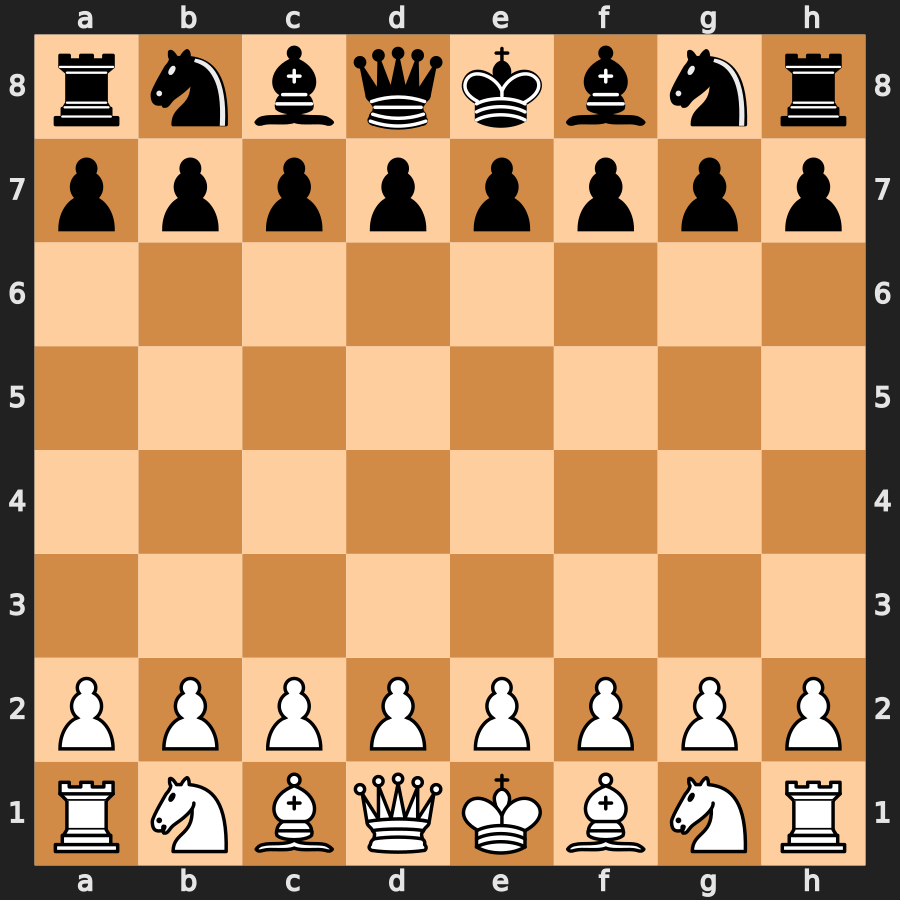
\includegraphics[width=0.35\textwidth]{rozdzialy/rozdzial01/1_komunikacja-z-systemem/rysunki/pozycja_startowa}
        &
        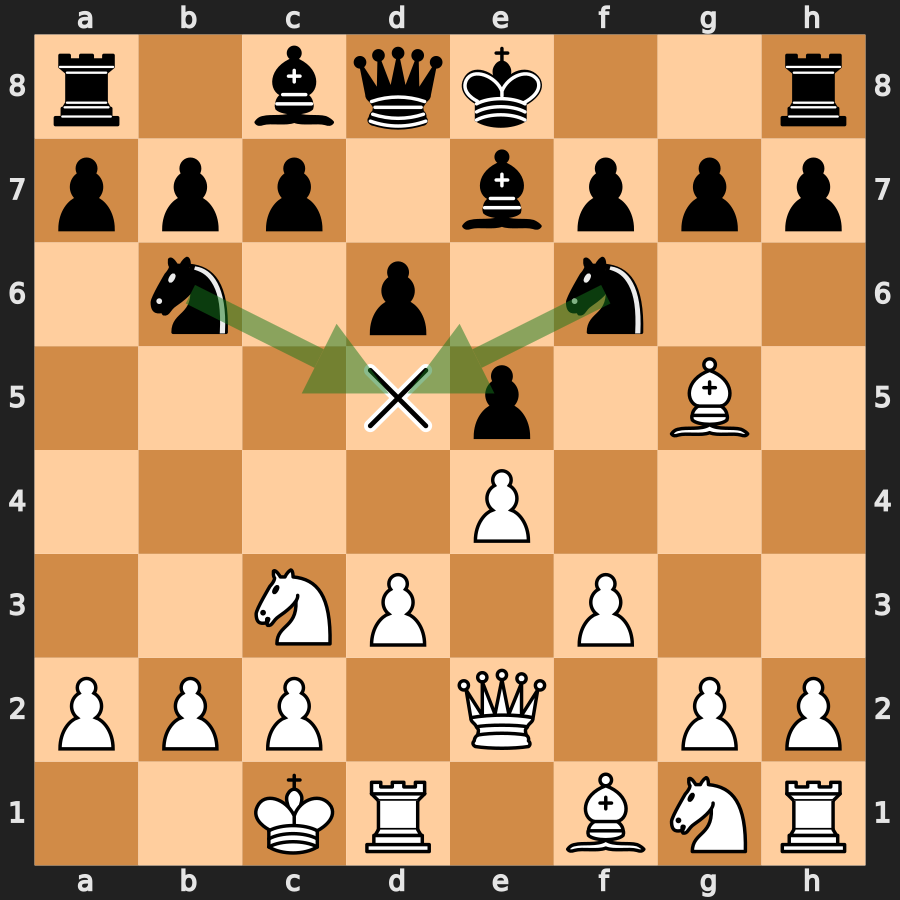
\includegraphics[width=0.35\textwidth]{rozdzialy/rozdzial01/1_komunikacja-z-systemem/rysunki/pozycja_niejasna}
    \end{tabular}
    \caption{Przykładowe pozycje szachowe: a) startowa, b) po paru ruchach}
    \label{fig: basic_chess_positions}
\end{figure}

\centerline{
    \ref{fig: basic_chess_positions} a) \lstset{basicstyle=\ttfamily}\lstinline{rnbqkbnr/pppppppp/8/8/8/8/PPPPPPPP/RNBQKBNR w KQkq - 0 1}
}
\centerline{
    \ref{fig: basic_chess_positions} b) \lstset{basicstyle=\ttfamily}\lstinline{r1bqk2r/ppp1bppp/1n1p1n2/4p1B1/4P3/2NP1P2/PPP1Q1PP/2KR1BNR b kq - 7 7}
}



\subsection{Szachowa Notacja Algebraiczna}
\label{subsec:notacja-algebraiczna}

Kluczowym aspektem, z perspektywy komunikacji z systemem, jest także określenie formatu zapisu ruchów.
W aplikacji wykorzystano Szachową Notację Algebraiczną.

Notacja ta, w swojej krótkiej formie, jest powszechnie stosowana w literaturze oraz podczas oficjalnych zawodów.
Stanowi jedyną formę zapisu posunięć uznawaną przez Międzynarodową Federację Szachową.
Jej zapis zawiera informacje o rodzaju ruszanej bierki oraz o jej polu docelowym.
Zapis ten z punktu widzenia komputerów zawiera jednak wadę.
W sytuacji, w której dwie bierki tego samego rodzaju mogą poruszyć się na jedno pole, występuje dwuznaczność zapisu.
Choć w takiej sytuacji dodaje się do ruchu kolumnę bądź wiersz startowy różniący obie bierki, jest to rozwiązanie wymagające implementacji dodatkowej logiki oraz wiedzy o stanie całej planszy.

Znacznie bardziej intuicyjne dla komputerów jest zastosowanie długiej wersji szachowej notacji algebraicznej.
Zawarte są w niej informacje o polu startowym oraz polu docelowym ruchu, usuwając tym samym ryzyko dwuznaczności.
Roszady oznaczano przez pola ruchu króla, natomiast do ruchów z promocją dopisano literę określającą rodzaj podmienionej figury.



\subsection{Uniwersalny Interfejs Szachowy}
\label{subsec:interfejs-szachowy}

Uniwersalny Interfejs Szachowy (ang.~\emph{Universal Chess Interface}, w~skrócie UCI) \cite*{UCIdoc} jest~ustandaryzowanym protokołem tekstowym, służącym do wymiany informacji pomiędzy różnymi programami szachowymi.
Jego implementacja pozwoliła na komunikację silnika szachowego z wybranymi interfejsami graficznymi oraz środowiskami testowymi.

UCI jest protokołem rozbudowanym, pozwalającym między innymi na rozgrywki innych wersji szachów niż europejskie, dla przykładu Chess960.
W silniku zaimplementowano jedynie te z komend, które konieczne były do rozegrania podstawowej partii mierzonej czasowo.


Metodę połączenia z dowolnym programem obsługującym UCI przedstawiono w dodatku \ref{ch:instrukcja-wdrozenia}.
Opisy komend oraz przykład wymiany informacji pomiędzy aplikacją a GUI zaprezentowano w~dodatku \ref{ch:protokol-uci}.

\input{rozdzialy/rozdzial01/1_komunikacja-z-systemem/4_zarządzanie-czasem}



\section{Reprezentacja pozycji}
\label {sec:reprezentacja-szachownicy}

\subsection{Reprezentacja szachownicy}
\label{subsec:reprezentacja-szachownicy}

Struktury danych, wybrane do reprezentacji szachownicy, w dużym stopniu determinują implementację funkcji generowania dostępnych ruchów, a co za tym idzie, bezpośrednio wpływają na wydajność całego silnika.
Z tego względu ich dobór musiał zostać odpowiednio zaplanowany, uwzględniając ogół architektury programu.
Po zapoznaniu się z proponowanymi w~literaturze rozwiązaniami, w projekcie zdecydowano się zastosować dwie redundantne techniki reprezentacji 64 pól szachowych.

Obie charakteryzują się odmiennymi właściwościami, znajdując zastosowanie dla innych algorytmów wewnątrz programu.
Różnią się one pod względem gęstości zawartych informacji, szybkości dostępu do danych oraz łatwości modyfikacji.
Jedna z nich skupia się na każdym z~pól~szachownicy (ang.~\emph{Square Centric}), druga natomiast bierze pod uwagę położenie konkretnych rodzajów bierek (ang.~\emph{Piece Centric}).

Przy procesie implementacji omawianego fragmentu należało zachować szczególną ostrożność, aby ciągłe aktualizowanie dwóch niezależnych struktur danych nie doprowadziło do~ich rozspójnienia, a co za tym idzie wprowadzenia trudnych do zdebugowania błędów.
Ryzyko ich pojawienia zostało zminimalizowane dzięki wprowadzeniu testów jednostkowych regularnie kontrolujących poprawność operacji podczas enumeracji drzewa gry.
\subsubsection{Tablica pól szachowych}

Naturalnym podejściem do reprezentacji szachownicy wydało się zastosowanie 64 elementowej tablicy, w której każde pole odpowiada konkretnemu miejscu na planszy.
W tej implementacji poszczególne bierki zostały zakodowane liczbami od 1 do 6, natomiast cyfry 0 i 8 odpowiednio reprezentują biały oraz czarny kolor.
W ten sposób, za pomocą pojedynczych bajtów, można określić zarówno typ figury, jak i jej kolor na danym polu.

Taka struktura danych jest szczególnie użyteczna, gdy konieczna jest szybka odpowiedź na~pytanie, czy na danym kwadracie znajduje się figura, a jeśli tak, to jaka.
Dzięki prostemu indeksowaniu tablicy dostęp do informacji o stanie pojedynczego pola jest bardzo efektywny.

Wada tej techniki objawia się w momencie, gdy wymagane jest odnalezienie wszystkich pól~zawierających konkretny typ figury.
W takim przypadku konieczna staje się iteracja całej tablicy, w celu zidentyfikowania odpowiednich miejsc.
Operacja ta, szczególnie przy~wielokrotnym wywołaniu, może znacząco obniżyć wydajność implementowanego algorytmu.

%\begin{lstlisting}[
%    language=Java,
%    style=JavaStyle,
%    caption=Implementacja reprezentacji szachownicy tablicą pól,
%    label=lst:pierwszy]
%
%    public byte[] board = new byte[64];
%
%    @Override
%    public void addPieceOnSquare(byte square, byte color, byte piece) {
%        board[square] = (byte) (color | piece);
%    }
%
%    @Override
%    public void deletePieceOnSquare(byte square, byte color, byte piece) {
%        board[square] = 0;
%    }
%
%\end{lstlisting}


\subsubsection{Tablice bitowe bierek}

W celu zaadresowania powyższych spowolnień zastosowana została technika reprezentacji szachownicy za pomocą tablic bitowych, powszechnie znanych w środowisku programistów szachowych jako ang.~\emph{Bitboards}.
Informacja o położeniu konkretnego typu bierki na planszy przechowywana jest w postaci tablicy liczb o rozmiarze 8 bajtów.

Implementacja ta wykorzystuje kodowanie 64 polowej tablicy szachowej w 64 pojedynczych bitach zmiennej.
Oznaczając figurę na danym polu za pomocą jedynki, a pozostałe pola jako zera, można w prosty sposób zawrzeć informacje o planszy w dwunastu pojedynczych słowach.
Pozycje bierek nie są natomiast jedyną informacją, którą można zakodować w tablicach bitowych.
Uprzednio policzone maski możliwych ruchów czy atakowanych pól, to tylko niektóre z możliwych zastosowań, które na późniejszych etapach implementacji znacznie przyspieszały obliczenia.

Powszechne użycie 64-bitowej architektury sprawiło, że operacje na danych takiej wielkości są bardzo efektywne, gdyż nie wymagają rozbicia instrukcji na mniejsze części.
Dodatkowym atutem jest także szybkość manipulacji danymi przez operatory bitowe takie jak negacja, koniunkcja, alternatywa wykluczająca czy przesunięcie bitowe.
Z reguły, a w szczególności na starszych procesorach, operacje bitowe są szybsze, niż ich odpowiedniki w postaci operacji arytmetycznych.

%\begin{lstlisting}[
%    language=Java,
%    style=JavaStyle,
%    caption=Implementacja reprezentacji szachownicy tablicami bitowymi bierek,
%    label=lst:drugi]
%    public void addPieceOnSquare(byte square, byte color, byte piece) {
%        bitBoards[piece | color] |= Long.rotateLeft(1L, square-1);
%    }
%
%    public void deletePieceOnSquare(byte square, byte color, byte piece) {
%        bitBoards[piece | color] &= ~Long.rotateLeft(1L, square-1);
%    }
%\end{lstlisting}



\subsection{Reprezentacja stanu}
\label{subsec:reprezentacja-stanu}

Reprezentacja stanu zawiera resztę informacji koniecznych do przedstawienia pozycji szachowej odkodowywanej z FEN.
Znajdują się w niej dane o możliwych roszadach, polu en-passant, liczbie posunięć od ostatniego bicia, czy informacji, do którego gracza należy następny ruch.

W tej klasie zawarto także informację o tym, jaki ruch doprowadził do aktualnej pozycji, oraz strukturę HashMap zawierającą informacje, jak często dane pozycja wystąpiły już w grze.
Pozwoliło to na wykrywanie trzykrotnego powtórzenia stanu gry (niekoniecznie następującego bezpośrednio po sobie), które skutkuje automatycznym remisem.

Przechowywanie danych o etapie gry oraz o wyliczonej ocenie heurystycznej pozwoliło na~uniknięcie wielokrotnego przeliczania tych samych wartości przez różne fragmenty programu.



\subsection{Reprezentacja ruchu}
\label{subsec:reprezentacja-ruchu}





\usepackage{biblatex}\section{Generowanie ruchów}
\label{sec:generowanie-ruchow}

Generowanie możliwych ruchów w danej pozycji jest jednym z podstawowych, ale~także~kluczowych elementów każdego silnika szachowego.
Jego efektywna implementacja to taka, w której silnik spędza jak najmniej czasu, pozostawiając możliwości obliczeniowe na~przeszukiwanie drzewa decyzyjnego.

Podstawowym rozróżnieniem stosowanych rozwiązań jest podział na generowanie ruchów pseudolegalnych oraz ruchów legalnych. \cite*{wiki-movegen}
Ruch pseudolegalny to taki, który nie narusza zasad ruchów poszczególnych bierek, natomiast istnieje ryzyko, że po jego wykonaniu własny król znajdzie się w szachu.
Takie rozwiązanie jest możliwe do zastosowania, z~uwagi na~pozostawienie odpowiedzialności za sprawdzenie legalności ruchu funkcji, która ten ruch wykonuje.
Główną zaletą tej metody jest znacznie łatwiejsza implementacja.

Kolejnym aspektem wartym zaznaczenia, jest wydzielenie oddzielnego generatora dla~ruchów zbijających.
Z perspektywy dalszej implementacji znacznie ułatwiło to rozwój silnika o ewaluacje stanów cichych oraz sortowanie ruchów, o czym wspomniano w następnym roździale.

\subsection{Operacje na mapach bitowych}
\label{subsec:operacje-na-mapach-bitowych}

\subsubsection{Generowanie ruchów piona}

Pion ma do dyspozycji parę możliwych ruchów, które należało zaimplementować: ruch o~jedno pole do przodu, ruch o dwa pola do przodu, bicie w lewo, bicie w prawo oraz ruch en-passant.
Każdy z graczy zaczyna rozgrywkę z ośmioma pionami, a w większości partii ich ilość pozostaje znaczna aż do zakończenia rozgrywki.
Czasochłonna wydawała się więc iteracja po~wszystkich bierkach tego typu i indywidualne generowanie ruchów dla każdego z osobna.
Z tego względu wykorzystano operacje bitowe i przesunięcia na masce bitowej.

Poniżej przykład generowania ruchów dla białych pionków.
\begin{align*}
    moves & = empty && \text{pole końcowe musi być puste} \\
    moves & = moves \wedge (P_w\ll16) && \text{pionek musi być dwa wiersze niżej}\\
    moves & = moves \wedge (empty\ll8) && \text{wiersz niżej musi być pusty}\\
    moves & = moves \wedge rank4 && \text{pole końcowe musi być w czwartym wierszu}
\end{align*}

\begin{figure}[ht]
    \centering
    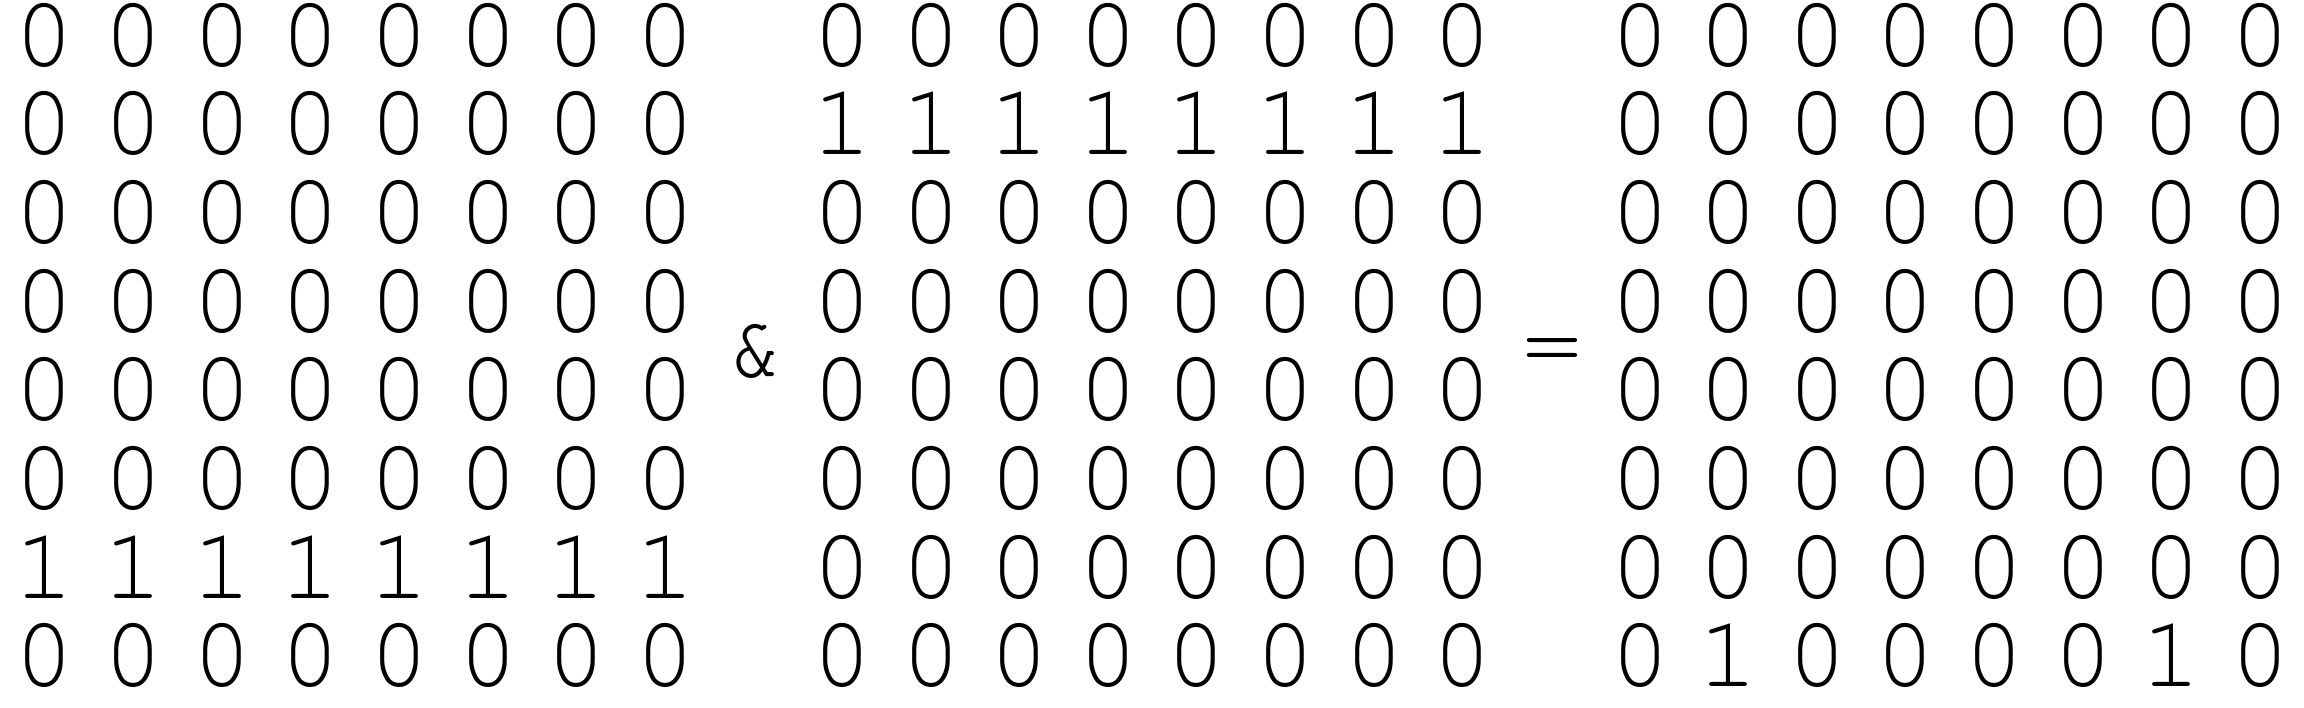
\includegraphics[width=0.85\linewidth]{rozdzialy/rozdzial01/3_generowanie-ruchow/rysunki/bitboards-arithmetic}
    \caption{Kodowanie ruchu szachowego}
    \label{fig:bitboards-arithmetic}
\end{figure}


\subsubsection{Generowanie ruchów hetmana, wieży i gońca}

Ruchy hetmana są połączeniem ruchów wieży oraz gońca, z tego względu można je generować w ten sam sposób.
Techniki te operują na bardzo podobnych zasadach, co generowanie ruchów piona, z tą różnicą, że figury mogą poruszać się o dowolną liczbę pól w danym kierunku, aż do momentu napotkania innej bierki na swojej drodze.
Aby uniknąć skomplikowanych obliczeń, należało zaimplementować funkcję, która w literaturze znana jest pod nazwą (ang.~\emph{Hyperbola Quintessence}).

$lineAttacks =   (o-2r) \string^ reverse( o'-2r')$

\subsubsection{Generowanie ruchów króla i skoczka}


\subsection{Hyperbola Quintessence}
\label{subsec:hyperbola-quintessence}

Generowanie ruchów hetmana, wieży i gońca odbywa się w sposób odmienny.
Wynika to~z~faktu, że figury te poruszają się~o~dowolną liczbę pól w danym kierunku, aż do momentu napotkania innej bierki na swojej drodze.
W przypadku bierki przeciwnika możliwe jest bicie, w przypadku bierki własnej, należy zatrzymać się pole wcześniej.
Choć są to trzy różne figury, to mają do dyspozycji dwa możliwe ruchy, ruch w linii prostej, jak wieża, oraz ruch po przekątnej, jak~goniec.
Ruchy hetmana są natomiast sumą dwóch powyższych generatorów.

Większość silników szachowych korzystających z masek bitowych implementuje funkcję, która w literaturze zwana jest jako ang. \emph{Hyperbola Quintessence}.
Pozwala ona na wygenerowanie dostępnych ruchów w jednej prostej oraz na uniknięcie zawiłej logiki iteracyjnej.
\begin{align*}
    o = \text{11010101} && o' = \text{10101011} && \text{pola zajęte przez bierki} \\
    r = \text{00010000} && r' = \text{00001000} && \text{pole figury dla której generujemy ruchy} \\
    o-r = \text{11000101} && o'-r' = \text{10100011} && \text{pola zajęte minus pole figury} \\
    \alpha = o-2r = \text{10110101} && \beta = o'-2r' = \text{10011011} && \text{pola zajęte dwukrotnie minus pole figury} \\
    (\alpha \oplus \beta') \wedge \neg \gamma && \text{01101100} && \text{maska legalnych ruchów}
\end{align*}
\begin{multicols}{2}
    \begin{itemize}[label={}]
        \item \(\oplus\) — alternatywa wykluczająca
        \item \(\wedge\) — koniunkcja
        \item \(x'\) — odwrócenie bitów
        \item \(\gamma\) — maska pól zajętych przez własne bierki
    \end{itemize}
\end{multicols}





\subsection{Ruchy specjalne}
\label{subsec:ruchy-specjalne}

Pozostałymi ruchami do zaimplementowania było bicie w przelocie oraz cztery roszady.
Z uwagi na znikomą liczbę takich posunięć w danej pozycji oraz na złożoną logikę tych ruchów, zostały one wygenerowane explicite z zasad gry.

Oba typy ruchów wymagały dodatkowej weryfikacji z danymi dostępnymi w reprezentacji stanu gry.
Pierwszy z nich – en-passant – został wygenerowany przez nałożenie na siebie maski pola bicia w przelocie oraz maski pionów, odpowiednio przesuniętych o $\pm 7$ oraz $\pm 9$ kratek.

Aby uzyskać prawo roszady, należy spełnić następujące warunki:
\begin{enumerate}
    \item Ani król, ani wieża biorąca udział w roszadzie nie mogły wykonać wcześniej ruchu.
    \item Pola między królem a wieżą muszą być puste.
    \item Król nie może znajdować się w szachu.
    \item Król nie może przechodzić bądź kończyć ruch na polach atakowanych przez bierki przeciwnika.
\end{enumerate}




\subsection{Generowanie ruchów legalnych}
\label{subsec:generowanie-ruchow-legalnych}

\subsubsection{Technika usuwania ruchów pseudo-legalnych}

Po zaimplementowaniu logiki opisanej powyżej, silnik był zdolny do generowania posunięć pseudolegalnych.
Natomiast ruch, po którym własny król znajduje się w szachu, nie tylko jest ruchem nieoptymalnym, ale również z punktu widzenia reguł FIDE nielegalnym.

W literaturze można znaleźć kilka podejść do problemu odfiltrowywania ruchów pseudolegalnych.
Niektóre z nich korzystają z dodatkowych masek bitowych, reprezentujących pola atakowane przez bierki danej strony.
W niniejszej implementacji zastosowano jednak rozwiązanie, w subiektywnym odczuciu autora, łatwiejsze.

Po wykonaniu konkretnego ruchu, w miejscu, gdzie znajduje się król, stawiane są kolejne figury oraz generowane są dostępne bicia.
Jeśli wśród bić znajduje się bierka przeciwnika, tego samego typu, co aktualnie podstawiona, oznacza to, że król znajduje się w szachu, a więc posunięcie nie należy do kategorii ruchów legalnych.

\subsubsection{Test wydajności}

Generatory ruchów szachowych posiadają skomplikowaną logikę.
Z tego względu bardzo łatwo o popełnienie błędu w implementacji.
Dopuszczenie choćby jednego błędu, skutkować będzie jego propagacją na większych głębokościach, a w skrajnych przypadkach doprowadzi do~zakończenia programu.

Ocena poprawności metodą przeprowadzania rozgrywek z silnikiem szachowym jest~rozwiązaniem czasochłonnym.
Odwiedzenie dużej ilości węzłów drzewa gry, w~celu~sprawdzenia poprawności wykonywania ruchów, jest praktycznie niemożliwe.
Błędy w~ten~sposób powstałe są trudne do zlokalizowania.

Z tego względu zastosowano Test Wydajności (ang.~\emph{Performance Testing}, w~skrócie Perft~Test).
Choć nazwa mogłaby wskazywać na testowanie prędkości generowanych ruchów, test ten można przeprowadzić także w celu kontroli poprawności.
Metoda ta~opiera się~na~wykorzystaniu algorytmu DFS dla ograniczonej głębokości na drzewie gry, przy jednoczesnym zliczaniu odwiedzonych węzłów.
Tak otrzymane wyniki można porównać z konsensusem osiągniętym przez twórców silników szachowych.
Jako punkt odniesienia autor przyjął wyniki generowane przez silnik Stockfish.
Przeprowadzenie testów z różnych pozycji startowych oraz dla~różnych głębokości pozwoliło na potwierdzenie poprawności implementowanego generatora, z~prawdopodobieństwem graniczącym z pewnością.
Przykładowe wyniki zaprezentowano w dodatku \ref{ch:wyniki-perft}.



\section{Ocena heurystyczna}
\label{sec:ocena-heurystyczna}

Funkcje heurystyczne są komponentami silnika szachowego, które odpowiadają za ocenę konkretnej pozycji szachowej, z punktu widzenia jednego z graczy.
Są one istotne ze~względu na~to, że umożliwiają silnikowi wybór i wykonywanie takich ruchów, które prowadzą do~osiągnięcia najkorzystniejszej z punktu widzenia silnika pozycji.

Z czysto teoretycznego punktu widzenia, nieskończona moc obliczeniowa pozwalałaby na~przeszukanie pełnego drzewa gry, a co za tym idzie, jedyną funkcją heurystyczną godną implementacji, byłaby funkcja zwracająca $1$ w przypadku wygranej, oraz $-1$ w~przypadku przeciwnym.
W rzeczywistości natomiast mnogość możliwych ruchów z każdej pozycji nakłada limit co do głębokości przeszukiwania i konieczności oceny pozycji, które nie~są~liśćmi drzewa, to jest pozycjami, które nie kończą partii.
Z tego względu konieczne było zaimplementowanie funkcji heurystycznych, które, choć nie prowadzą gracza bezpośrednio do~wygranej, to~przybliżają go do tego celu na określone sposoby.

W podstawowej wersji silnika zaimplementowano dwie funkcje heurystyczne.

Funkcja zerowa, która zwraca $MAX$ w przypadku mata króla przeciwnika, $MIN$ w~przypadku mata własnego króla, oraz $-5000$ w przypadku remisu wynikającego z~trzykrotnego powtórzenia pozycji bądź reguły 50 ruchów.
Celem było demotywowanie silnika do~wykonywania ruchów prowadzących do remisu.

Funkcja pierwsza, która opiera się na~intuicyjnym założeniu, że korzystniejsza pozycja to~taka, w której gracz ma więcej bierek na planszy niż~przeciwnik.
Różnica między liczbą bierek konkretnego typu dla gracza oraz jego oponenta jest przemnażana przez jej wagę.
W~tym celu skorzystano ze skali zaproponowanej przez Claude Shannona, w której odpowiednio hetman, wieża, goniec, skoczek oraz pion mają wartości: 900, 500, 300, 300 oraz 100.

W dalszej części pracy przedstawiono kolejne funkcje heurystyczne, mające na celu poprawę precyzji oceny pozycji.
Klasa oceny heurystycznej silnika szachowego zwraca ocenę pozycji~$P$~dla koloru, który aktualnie wykonuje ruch według zasady:

\begin{equation}
    Ocena(P) =
    \begin{cases}
        H_0(P) & \text{if } H_0(P) \ne 0 \\
        $\sum\limits_{i=1}^{n} (c_i \cdot H_i(P))$ & \text{else}\\
    \end{cases}
\end{equation}
gdzie,
\begin{multicols}{2}
    \begin{itemize}[label={}]
        \item \(H_0\) – heurystyka końca gry
        \item \(H_i\) – kolejne funkcje heurystyczne
        \item \(c_i\) – waga heurystyki $i$
    \end{itemize}
\end{multicols}

Manipulowanie wagami konkretnych heurystyk pozwoliło na przeprowadzenie testów porównawczych i ich dostrojenie w celu uzyskania jak najdokładniejszej oceny.



\usepackage{biblatex}\section{Algorytm wyszukiwania}
\label {sec:algorytm-wyszukiwania}

W 1950 roku Amerykański matematyk Claude Shanon opublikował pracę naukową zatytułowaną \("\)Programowanie komputera do gry w szachy\("\)\cite*{Shannon1950XXIIPA}.
Praca ta stała się teoretyczną podstawą tworzenia silników szachowych.
Zawiera ona między innymi oszacowanie co do ilości możliwych pozycji szachowych, wynoszące $10^{43}$.
Choć oszacowanie to zmieniało się w pewnym stopniu na przestrzeni lat, to jednak liczba ta dowodzi jednoznacznie, że z uwagi na skalę problemu nie jest możliwa implementacja tablicy zawierającej wszystkie pozycje szachowe, oraz najlepsze możliwe na nie odpowiedzi.
Koniecznym było zaimplementowanie algorytmu, który dla konkretnej strategii, decydowałby jaki ruch wykonać uwzględniając daną głębokość drzewa decyzyjnego.


\subsection{Algorytm min-max \colorbox{yellow}{Implemented}}
\label{subsec:algorytm-min-max}


\subsection{Iteracyjne pogłębianie wyszukiwania}
\label{subsec:iteracyjne-pogebianie-wyszukiwania}

Lorem ipsum dolor sit amet, consectetur adipiscing elit

\subsection{Zarządzanie czasem \colorbox{yellow}{Implemented}}
\label{subsec:zarzadzanie-czasem}



\chapter{Ulepszenia dla silnika szachowego}
\label{ch:ulepszenia-dla-silnika-szachowego}

Po opisanych w rozdziale drugim krokach silnik stał się zdolny do samodzielnej gry.
W poniższej części opisane zostały zagadnienia związane z poprawą szybkości i precyzji działania systemu.
W pierwszej kolejności skupiono się na ulepszeniu przeszukiwania ruchów w celu znalezienia najlepszego z posunięć.
Następnie opisano zmiany heurystyki planszy pozwalające silnikowi na~lepszą ocenę bieżącej sytuacji gry.

\section{Ulepszenia dla wyszukiwania}
\label{sec:ulepszenia-dla-wyszukiwania}


\subsection{Biblioteka otwarć}
\label{subsec:biblioteka-otwarc}

\subsubsection{Opis zagadnienia}
Głównym problemem, który należało rozwiązać, były otwarcia partii rozgrywanych przez silnik.
Gry szachowe zawsze rozpoczynają się z tego samego położenia, więc wiadomo, że~system znajdzie się w wielu pozycjach bezpośrednio wynikających z pierwszych posunięć.
Program natomiast poświęcał na obliczenia wiele czasu, który lepiej byłoby spożytkować w~środkowym etapie rozgrywki.

Profesjonalni gracze, korzystając z dorobku i doświadczenia wielu pokoleń szachistów, zapamiętują pierwsze posunięcia do wykonania.
Tym samym oszczędzają czas, który pozostaje na bardziej złożone pozycje w środkowej fazie gry.

\subsubsection{Implementacja}
W celu zaimplementowania biblioteki otwarć, dostępne posunięcia czytane są z pliku, a~następnie zapisywane przy inicjalizacji silnika do HashMapy \texttt{<String, []Moves>}.
Podczas działania silnika, FEN aktualnej pozycji porównywalny jest z dostępnymi kluczami, a ruch losowo wybierany spośród dostępnych w tablicy.
W przypadku nieznalezienia klucza program przechodzi do gry środkowej z wykorzystaniem algorytmu negaMax.

W literaturze znanych jest wiele formatów zapisu biblioteki otwarć, np.\ EPD, PGN czy~Bin-format.
System wykorzystuje bibliotekę wygenerowaną przez Sebastiana Lague i~dostępną na licencji MIT w~implementacji jego silnika~\cite*{opening-library}.
\subsubsection{Rezultat}
Efektem prac stał się silnik, który początkowe posunięcia wykonuje za pomocą podpiętej biblioteki otwarć.
Dzięki temu pierwsze ruchy wykonywane są bardzo szybko, pozostawiając cenny czas obliczeniowy na dalszą grę, tym samym zwiększając precyzję.

We wcześniejszej wersji silnik był deterministyczny, to jest, dla konkretnej głębokości i pozycji, algorytm zwracał ten sam najlepszy ruch.
Dodatkowym atutem stała się jego nieprzewidywalność.
Początkowe posunięcia są zrandomizowane, co pozwala na jego testowanie w większej ilości wariantów, a także umila rozgrywkę użytkownikowi.

\subsection{Alfa-Beta cięcie}
\label{subsec:alfa-beta-ciecie}
\subsubsection{Opis zagadnienia}
Poprawne wykonanie algorytmu negaMax nie gwarantuje jego skuteczności.
Wraz z~pogłębianiem wyszukiwania rośnie również liczba wierzchołków, które należy odwiedzić.
Uśredniając, liczba dzieci, to jest pozycji wynikających z wykonania ruchu, dla danego rodzica w szachach wynosi $35$. \cite*{branching-factor}
Własność ta nazywa się współczynnikiem rozgałęzienia (ang.~\textit{branching~factor}).

Do minimalizacji liczby odwiedzonych węzłów wykorzystuje się alfa-beta cięcia.
Jest to przykład algorytmu metody podziału i ograniczeń, a jego skuteczność w dużym stopniu zależy~od kolejności przeszukiwanych ruchów.
Zakładając ułożenie posunięć od najlepszego, algorytm wykona najwięcej cięć, co w efekcie skutkować będzie zmniejszeniem liczby odwiedzonych wierzchołków dla głębokości według wzoru z tabeli:

\begin{table}[htb] \small
\centering
\caption{Teoretyczny limit alfa-beta cięcia dla współczynnika rozgałęzienia $b_f = 35$}
\label{tab:alfa-beat}
\renewcommand{\arraystretch}{1.5}
\begin{tabular}{|c|c|c|}\hline
Głębokość $n$ & ${b_{f}}^{n}$ & $b_{f}^{\lceil \frac{n}{2} \rceil} + b_{f}^{\lfloor \frac{n}{2} \rfloor} - 1$\\ \hline\hline

$1$ & $35$ & $35$\\ \hline
$2$ & $1225$ & $69$\\ \hline
$3$ & $42 875$ & $1259$\\ \hline
$\vdots$ & $\vdots$ & $\vdots$\\ \hline
$10$ & $2,76 * 10^{15}$ & $1,05 * 10^{8}$\\ \hline

\end{tabular}
\end{table}

Posortowanie ruchów od najgorszych, spowoduje brak możliwych cięć, a tym samym wynik będzie identyczny, jak przy algorytmie bez implementacji alfa-beta cięcia.


\subsubsection{Implementacja}

Algorytm alfa-beta cięcia jest edycją kodu funkcji negaMax \ref{lst:drugi}.
$\alpha$ oraz $\beta$ zostają dodane jako argumenty.
W sytuacji, gdy \texttt{score} $>$ \texttt{bestMoveValue} oraz $\alpha >$ \texttt{bestMoveValue}, $\alpha$~zostaje zaktualizowana na \texttt{bestMoveValue}.
Jeśli \texttt{score} $>=\beta$ następuje odcięcie i zwracana jest wartość \texttt{bestMoveValue}.
W wywołaniach funkcji na większej głębokości $\alpha = -\beta$ oraz $\beta = -\alpha$.

\subsubsection{Rezultat}

Implementacja powyższego rozwiązania pozwoliła na zmniejszenie liczby odwiedzonych wierzchołków podczas przeszukiwania, a tym samym pozwoliła iteratywnemu pogłębianiu na~osiągnięcie lepszych rezultatów.
Realna wartość tego ulepszenia jest różna w zależności od~aktualnej pozycji na szachownicy.
\subsection{Ewaluacja stanów cichych}
\label{subsec:ewaluacja-cichych-stanow}

\subsubsection{Opis zagadnienia}
Silnik znacznie przyspieszył znajdowanie ruchów dla danej głębokości.
Zdarzały się jednak sytuacje, że zwracane wyniki znacznie odbiegały od optymalnych.
Dla przykładu mogła zdarzyć się sytuacja, że liściem w drzewie było bicie hetmanem skoczka \cite*{duch}.
Silnik zwracał wynik heurystyki jako bardzo wysoki i wykonywał powyższy ruch.
Program nie brał jednak pod uwagę faktu, że~na~głębokości o jednej większej, hetman ten mógłby zostać zbity przez wrogiego pionka.

Taką sytuację nazywa się efektem horyzontu.
Rozwiązaniem wykonywania nieoptymalnych ruchów, było wykonanie dodatkowego wyszukiwania po osiągnięciu głębokości końcowej.
Z liścia drzewa, które poprzednio zostało oceniane heurystycznie, wyprowadzono kolejne wyszukiwanie, w którym generowane ruchy są tylko biciami.
Pozwoliło to na ocenę tak zwanych stanów cichych, czyli pozycji, gdzie nie ma żadnego dostępnego ruchu, który prowadziłby do~bicia.

\subsubsection{Implementacja}

Algorytm rozwiązujący efekt horyzontu w literaturze nosi nazwę Quiescence Search.

\begin{lstlisting}[
    language=Java,
    style=JavaStyle,
    caption=Implementacja algorytmu Quiescence Search,
    label=lst:trzeci]
    public search(depth, alpha, beta) {
        standPat = evaluator.evaluate();
        if (depth == 0) return standPat;

        if (standPat >= beta) return beta;
        if (alpha < standPat) alpha = standPat;

        moves = generator.generateCaptureMoves();
        for(Move move : moves) {
            board.makeMove(move);
            score = -search(depth-1, -beta, -alpha);
            board.unmakeMove();

            if(score >= beta) return beta;
            if(score > alpha) alpha = score;
        }
        return alpha;
    }
\end{lstlisting}

Niektóre wersje tego algorytmu, oprócz ruchów prowadzących do bicia, korzystają także z~roszad, czy~podwójnych ruchów piona, z uwagi na ich szczególny charakter.

\subsubsection{Rezultat}

W efekcie implementacji algorytmu osiągnięto silnik, który jest odporny na efekt horyzontu.
Z reguły, dodatkowe wyszukiwanie prowadzi do odwiedzenia większej liczby węzłów niż~w~przypadku zwykłego wyszukiwania.
Co warte zaznaczenia, w niektórych przypadkach, chociażby wskazanych w dodatku \ref{ch:wyniki-perft}, algorytm Quiescence Search w połączeniu z~alfa beta cięciem skutkował zmniejszeniem liczby odwiedzonych węzłów.
Ostatecznie, czy~korzystniejszym jest wyszukiwanie dla większych głębokości, czy korzystanie wyłącznie ze~stanów cichych, zależy od konkretnej sytuacji na planszy.
%\subsection{Statyczne sortowanie ruchów}
\label{subsec:sortowanie-ruchow}

\subsubsection{Opis zagadnienia}
W czasie testów zauważono, że podczas przeszukiwania drzewa nie następuje taka ilość alfa-beta cięć, która pozwalałaby na znaczne przyspieszenie obliczeń.
Rozpoczynanie przeszukiwania węzłów gry od najlepszych posunięć pozwoliłoby na osiągnięcie teoretycznego limitu wskazanego w tabeli \ref{tab:alfa-beat-limit}.
W żaden sposób nie ma jednak możliwości wskazania, który z~dostępnych ruchów prowadzi do najlepszej pozycji, przed wykonaniem tych ruchów.
Istnieją jednak posunięcia, które można rozważyć w pierwszej kolejności, ze względu na ich szczególny charakter, a~tym~samym przyspieszyć cięcie.
Jeśli sortowanie jest niezależne od wcześniejszych obliczeń, to~jest to sortowanie statyczne.

\subsubsection{Implementacja}
Sortowanie wykonano dzięki implementacji interfejsu \texttt{Comparator} w klasie \texttt{Move}.
W celu porównania pomiędzy sobą dwóch dowolnych ruchów wykorzystano następujące założenia:
\begin{itemize}
    \item Ruch, który umożliwia bicie, jest prawdopodobnie lepszy od ruchów, które nie umożliwiają bicia.
    \item Wszystkie ruchy specjalne, takie jak roszady, podwójne ruchy pionem czy promocje, są lepsze od ruchów zwykłych.
    \item Promocje do wieży i gońca należy rozważyć na końcu, gdyż są mniej wartościowe od promocji do hetmana, jednocześnie dając dostęp do tych samych ruchów.
    \item Zastosowano technikę Najbardziej wartościowa ofiara – Najmniej wartościowa atakujący (ang.~\emph{Most Valuable Victim – Least Valuable Attacker}, w~skrócie MVV-LVA). Sortuje ona~bicia zakładając, że korzystniejsze są posunięcia, w których różnica pomiędzy wartością reprezentowaną przez bierkę bijącą a bierką zbitą, jest jak największa.
\end{itemize}

\subsubsection{Rezultat}
Dzięki zastosowaniu sortowania statycznego, udało się zwiększyć ilość alfa-beta cięć, co~skutkowało możliwością przeszukiwania drzew gry do większych głębokości.
Szczególnie zauważalne było to ulepszenie w procesie wyszukiwania stanów cichych, gdzie każdy z~dostępnych ruchów można było zakwalifikować za pomocą MVV–LVA.
Dodatek \ref{ch:wyniki-perft} zawiera przykładowe pozycje, w których porównano wyniki perft dla wersji klasycznej, z alfa-beta cięciem, oraz z sortowaniem ruchów.
%\usepackage{biblatex}\subsection{Tabela transpozycji}
\label{subsec:tabela-transpozycji}

\subsubsection{Opis zagadnienia}
Silnik szachowy wielokrotnie znajduje się w tej samej pozycji planszy, musząc wyliczać wartości heurystyczne od nowa.
Dzieje się tak, zarówno w przypadku dotarcia do pozycji w wyniku odmiennych sekwencji ruchów, jak i w wyniku szukania kolejnego ruchu po~ruchu przeciwnika.
Rozwiązaniem tego problemu jest zastosowanie tabeli transpozycji, która przechowuje wyniki obliczeń dla pozycji, mając jednocześnie na uwadze głębokość, dla~której wynik został obliczony.
W sytuacji, gdy silnik ponownie napotka na tę samą pozycję, w~pierwszej kolejności sprawdzi, czy w tabeli nie znajduje się już obliczony wynik dla tej samej, bądź większej głębokości.

\subsubsection{Implementacja}
Do implementacji tabeli transpozycji zastosowano strukturę \texttt{LinkedHashMap}, dla której kluczami są wartości \texttt{Zobrist Hasz} planszy, a wartościami struktura zawierająca wynik obliczeń dla danej pozycji oraz głębokość.
W trakcie działania programu silnik przechodzi przez miliony możliwych pozycji, natomiast możliwości przechowywania wyników są ograniczone.
W przypadku przekroczenia z góry ustalonego limitu wpisów usuwane są te wartości, które zostały użyte najdawniej.
Pozwala to na pozbycie się poddrzew, w których silnik nie będzie miał okazji się ponownie znaleźć, przy jednoczesnym zachowaniu prostoty implementacji.

W algorytmie negaMax z zaimplementowanym alfa-beta cięciem, istotna jest nie tylko informacja o dokładnej wartości pozycji, ale także o górnej i dolnej granicy tej wartości.
Taka~wersja została zaimplementowana w kodzie, wzorując się na pracy Dennisa Breukera~\cite*{transposition-phd}.

\subsubsection{Rezultat}
Po zastosowaniu ulepszenia zaobserwowano zmniejszenie liczby odwiedzonych węzłów w trakcie przeszukiwania drzewa gry.
Było to szczególnie widoczne przy mniejszych głębokościach, gdzie w dużej mierze pozycje zostały już wyliczone w trakcie poprzednich posunięć.

%\subsection{Okno estymacji}
\label{subsec:okno-estymacji}
\textit{Przyspiesza alpha-beta cięcie.}


\subsubsection{Opis zagadnienia}
\subsubsection{Implementacja}
\subsubsection{Rezultat}
%\subsection{Rozszerzanie wyszukiwania}
\label{subsec:rozszerzanie-wyszukiwania}

\subsubsection{Opis zagadnienia}
Rozszerzenie wyszukiwania to technika, która zakłada, że niektóre z dostępnych posunięć wymagają dodatkowego zbadania.
W przypadku, gdy taki ruch nastąpi, algorytm przeszukiwania przedłuży przeszukiwanie poddrzewa gry o jeden poziom.
W odróżnieniu od~Quiescence Search rozszerzenie wyszukiwania przedłuża się na wszystkie z dostępnych ruchów z pozycji, a nie tylko na te, które prowadzą do bicia.

\subsubsection{Implementacja}
Zdecydowano się na implementację dwóch rodzajów przedłużeń:
\begin{itemize}
    \item Jeśli ruch jest atakiem powodującym wystąpienie szacha, to przeszukiwanie zostaje przedłużone o jeden poziom.
    \item W przypadku, gdy istnieje jedynie jedno dostępne posunięcie, również przeszukiwanie zostaje przedłużone o jeden poziom.
\end{itemize}
W celu uniknięcia zbytniego rozgałęziania się drzewa, przedłużenie wyszukiwania może nastąpić w danym poddrzewie gry tylko raz.
\subsubsection{Rezultat}
W toku gry nie zaobserwowano znacznego wzrostu bądź spadku siły silnika.

%\subsection{Dynamiczne sortowanie ruchów}
\label{subsec:dynamiczne-sortowanie}
\begin{center}
    \textcolor{red}{\textbf{BEZ IMPLEMENTACJI, SAM OPIS}}
\end{center}


\subsubsection{Opis zagadnienia}


\section{Ulepszenia dla oceny heurystycznej}
\label{sec:ulepszenia-dla-oceny-heurystycznej}

\subsection{Tablice figur}
\label{subsec:tablice-figur}

\subsubsection{Opis zagadnienia}
Istotnym z punktu widzenia heurystyki silnika jest prawidłowa ocena informacji na planszy.
Ograniczona wiedza, jedynie co do ilości figur na planszy, była niewystarczająca, aby móc prowadzić rozgrywkę na odpowiednio wysokim poziomie.

Wraz z rozwojem strategii szachowych gracze wypracowali szereg schematów, które ułatwiają im podejmowanie decyzji, niezależnie od konkretnej sytuacji na planszy.
Są nimi między innymi: zajęcie centralnych pól przez pionki, nierozwijanie skoczka na skrajne pola planszy, czy pozycjonowanie wież na otwartych liniach i wierszach pionów przeciwnika.

\subsubsection{Implementacja}
Implementacja każdego z powyższych, jak i wielu innych reguł mogłaby okazać się czasochłonna i złożona obliczeniowo.
Zdecydowano się zatem na zastosowanie tablic figur, które można rozumieć jako mapy cieplne, reprezentujące korzystność umieszczenia figury na danym polu.
Dla każdego typu bierki ($2*6$) stworzono tablicę 64 elementową określającą wartości, odnośnie do tego, jak korzystne jest umieszczenie figury na danym polu.
Zastosowano się na nie tworzenie własnych tablic, a zastosowanie gotowych, dostępnych na forum tworzenia silników szachowych. \cite*{wiki-tablica-figur}

\begin{figure}[ht]
    \centering
    \begin{tabular}{@{}ll@{}}
        a) & b) \\
        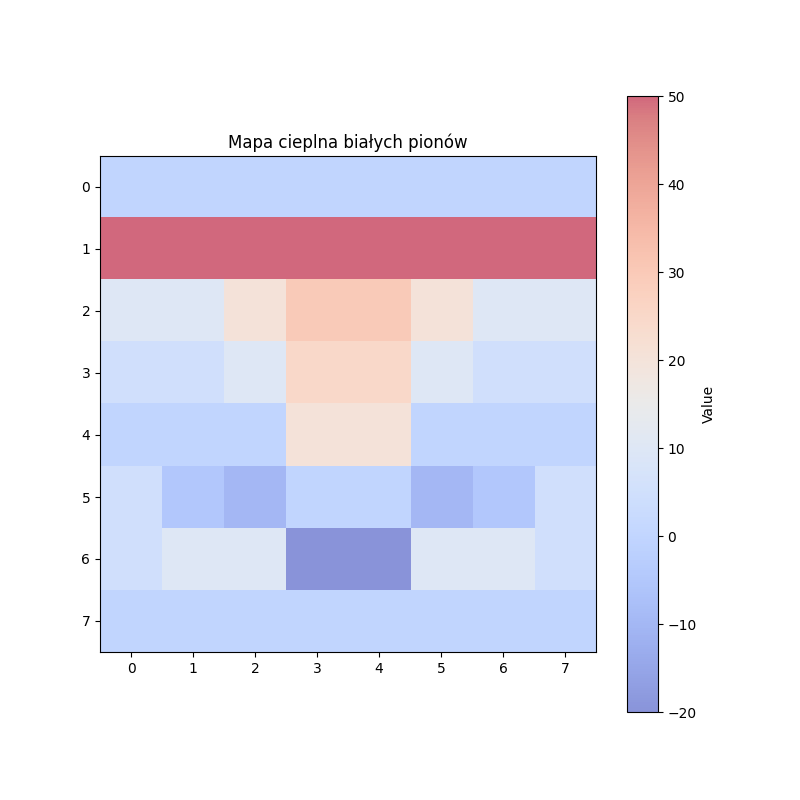
\includegraphics[width=0.5\textwidth]{rozdzialy/rozdzial02/2_ulepszenia_oceny/rysunki/bialePiony}
        &
        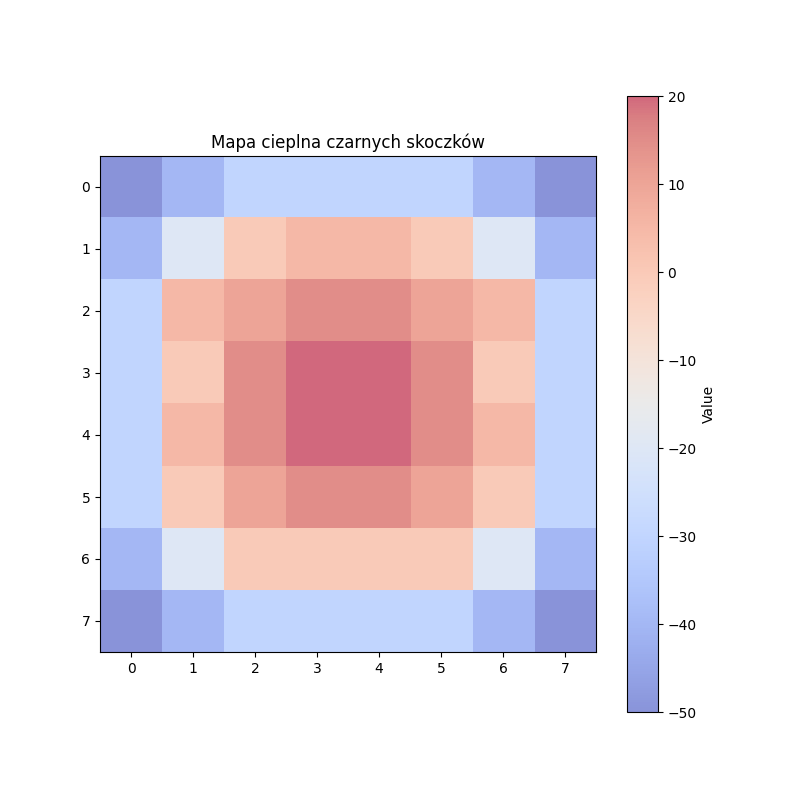
\includegraphics[width=0.5\textwidth]{rozdzialy/rozdzial02/2_ulepszenia_oceny/rysunki/czarneSkoczki}
    \end{tabular}
    \caption{Przykładowe tablice cieplne bierek: a) białych pionów, b) czarnych skoczków}
    \label{fig: tablice-figur}
\end{figure}

Rezultatem zastosowania tablic figur stał się silnik, który w odczuciu autora znacznie lepiej \enquote{rozumiał} pozycję na planszy.
\subsection{Ochrona króla}
\label{subsec:ochrona-krola}

{
    \color{red}
    \large Sprawdzanie, czy król jest chroniony, na przykład przez piony
}
\subsection{Struktura pionów}
\label{subsec:struktura-pionow}

\subsubsection{Opis zagadnienia}
Po implementacji ulepszenia \ref{subsec:tablice-figur} silnik zyskał zdolność oceny pozycyjnej.
Niedoskonałością było natomiast, że bierki oceniane były pojedynczo, to jest bez uwzględnienia ich wzajemnych relacji, oraz relacji w stosunku do bierek przeciwnika.
Było to szczególnie przydatne w przypadku pionków.
Termin \enquote{struktura pionów} jest szeroko znany w literaturze szachowej \cite*{stuktura-pionow} i odnosi się do technik mających na celu skoordynowaną obronę własnej części szachownicy oraz przeprowadzania ataków z wykorzystaniem pionów.
Skuteczne pozycjonowanie pionków na planszy może prowadzić do uzyskania przewagi w grze.

\subsubsection{Implementacja}
Zasady rozumiane przez graczy szachowych w sposób intuicyjny należało przekształcić na zbór reguł możliwych do zrozumienia przez program, a prowadzących do skutecznej oceny pozycji.
\begin{itemize}
    \item Pionki, które posiadają z tyłu po swojej prawej lub lewej stronie innego pionka, są uważane za dobrze chronione.
    \item Pionki nieposiadające za sobą innych pionków na sąsiednich kolumnach są traktowane jako izolowane i trudne do obrony.
    \item Dwa pionki znajdujące się w jednej linii pionowej (tzw. \enquote{zdublowane}) są uważane za~małowartościowe, gdyż odsłaniają inne linie na potencjalne ataki.
    \item Pionki, dla których istnieje możliwość promocji, spowodowana brakiem pionów przeciwnika na sąsiednich kolumnach, są uznawane za bardzo wartościowe.
\end{itemize}

Powyższe techniki zostały w dużej mierze zaimplementowane z wykorzystaniem uprzednio zainicjowanych tablic bitowych bierek i operacjach na nich.
Odbyło się to w sposób analogiczny do generowania dostępnych ruchów.

\subsubsection{Rezultat}
Rezultatem stał się silnik, który w sposób bardziej złożony oraz koherentny był w stanie ocenić swoją sytuację na planszy.
Istniało natomiast ryzyko, że czas konieczny na przeprowadzanie koniecznych obliczeń znacząco przewyższy oferowane korzyści.
Nie sposób było to sprawdzić w trakcie zwykłej gry przeciw silnikowi.
Rzeczywiste efekty przedstawiono w rozdziale \ref{ch: ocena-sily-silnika}.
%\subsection{Moment gry \colorbox{red}{TODO}}
\label{subsec:moment-gry}

{
    \color{red}
    \large Początek - środek - koniec.
    Różne wartości, szczególnie dla króla w zależności od momentu gry.
}
\subsection{Mobilność}
\label{subsec:mobilnosc}
\textit{Usprawnia pozycjonowanie hetmana, wieży i gońca.}


\subsubsection{Opis zagadnienia}
\subsubsection{Implementacja}
\subsubsection{Rezultat}
%\subsection{Algorytm genetyczny}
\label{subsec:genetyczny}
\begin{center}
    \textcolor{red}{\textbf{BEZ IMPLEMENTACJI, SAM OPIS}}
\end{center}

\subsubsection{Opis zagadnienia}





\chapter {Ocena siły silnika}
\label {ch: ocena-sily-silnika}

Zastosowane w poprzednim rozdziale ulepszenia w postaci heurystyk oraz algorytmów przeszukiwania drzewa w empirycznym odczuciu autora przynosiły zamierzone rezultaty.
W~celu potwierdzenia tych przypuszczeń konieczne było przeprowadzenie bardziej formalnych, to jest miarodajnych i obiektywnych, testów.

\section {Porównanie wersji silnika}
\label {sec: porownanie-wersji-silnika}

W pierwszej kolejności wysiłki skierowano ku porównaniu wersji silnika z różnym poziomem zaimplementowanych usprawnień.
Pozwoliło to na potwierdzenie poprawności zaimplementowanych rozwiązań oraz na wyłonienie jego najsilniejszej wersji.

\subsection{Ustalona liczba rozgrywek}
\label{subsec:ustalona-liczba-rozgrywek}

Najbardziej oczywistą, a zarazem najłatwiejszą do zaimplementowania metodą porównawczą jest rozegranie określonej liczby pojedynków pomiędzy oponentami, a następnie sprawdzenie współczynnika wygranych.
Do przeprowadzenia testów wykorzystano program komputerowy Cutechess, służący nie tylko jako szachowy interfejs graficzny, ale także jako zarządca turniejowy dla silników implementujących protokół UCI.
Pomiędzy każdą parą silników rozegrano po 25 gier, każda trwająca 1 minutę na partię plus 0,6 sekundy na ruch.

Co zaobserwowano w wynikach przedstawionych na rysunku \ref{fig:wyniki-wersje}, to fakt, że zastosowane ulepszenia w postaci heurystyk oraz algorytmów przeszukiwania drzewa, przyniosły zamierzone rezultaty.
Wersja silnika z zaimplementowanymi ulepszeniami wygrywała znaczącą większość pojedynków z poprzednią wersją oraz z podstawowym programem.

\subsubsection{Najkorzystniejsze ulepszenia}

Największe różnice zaobserwowano w ulepszeniach:
\begin{itemize}
    \item \textbf{Tablica figur} – współczynnik wygranej dla tego ulepszenia sięgnął 90\%.
    Wynikło to po części z tego, że silnik uzyskał o wiele więcej informacji co do pozycjonowania konkretnych figur na planszy.
    Z drugiej strony mogło to wynikać z przewidywalności ruchów z uwagi na determinizm silnika.
    Po zaimplementowaniu tablicy otwarć gry były bardziej losowe.
    \item \textbf{...} – lorem ipsum dolor sit amet, consectetur adipiscing elit.
\end{itemize}

\subsubsection{Najmniej istotne ulepszenia}
Najmniejsze różnice zaobserwowano natomiast w ulepszaniach:
\begin{itemize}
    \item \textbf{Ochrona króla} – wersja ulepszona, jak i poprzednia otrzymały po 50\% wygranych.
    Przypuszczeniem autora jest, że zmiana heurystyki dotyczyła bardzo specyficznych sytuacji, które nie miały dużego wpływu na ogół rozgrywek.
    \item \textbf{...} – lorem ipsum dolor sit amet, consectetur adipiscing elit.
\end{itemize}

\begin{figure}[ht]
    \centering
    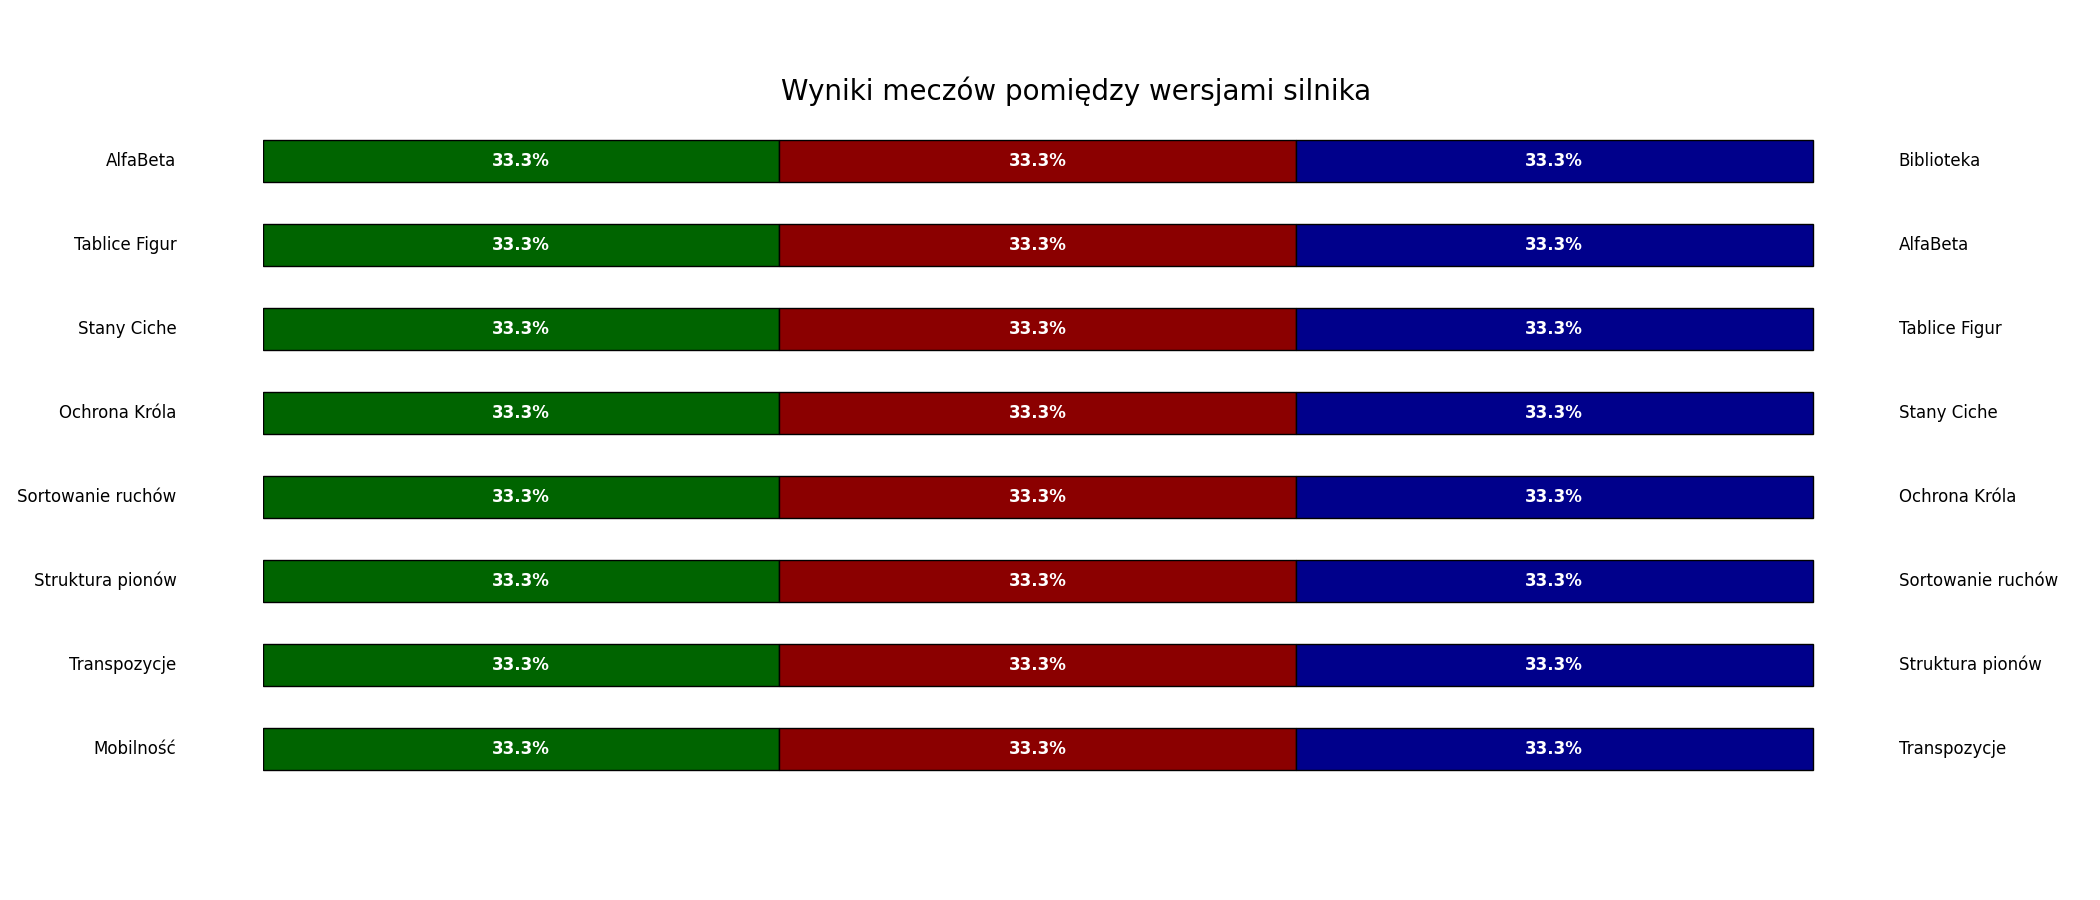
\includegraphics[width=1\linewidth]{rozdzialy/rozdzial03/1_porownanie-wersji-silnika/rysunki/gry-wyniki}
    \caption{Wyniki rozgrywek pomiędzy wersjami silnika}
    \label{fig:wyniki-wersje}
\end{figure}

\subsection{Sequential Probability Ratio Test}
\label{subsec:sequential-probability-ratio-test}
Testy porównawcze stosujące ustaloną liczbę rozgrywek, miały jednak szereg wad wpływających na wyniki testów.
Przede wszystkim, nie sposób było w tej metodzie ustalić, ile partii należy rozegrać, aby uzyskać wiarygodne statystycznie wyniki.
W przypadku dużej przewagi jednego z silnika wyniki można było uznać za autentyczne, jednak przy mniejszych różnicach powstawało ryzyko, że rozgrywki nie były reprezentatywne.

W celu zwiększenia wiarygodności wyników, zdecydowano się na zastosowanie Sekwencyjnych Testów Probabilistycznych (ang.\ \emph{Sequential Probability Ratio Test}, SPRT).
\subsubsection{Metodologia}
    Who knows? I dont.
\subsubsection{Przeprowadzenie testów}
    W celu przeprowadzenia SPRT zdecydowano się na ponowne zastosowanie Cutechess.
\subsubsection{Omówienie wyników}
\newpage
\section {Porównanie z innymi silnikami}
\label {sec: porownianie-z-silnikami}

Przedstawione powyżej rozwiązania są w stanie z dużą dozą pewności wskazać najsilniejszą wersję silnika szachowego.
Są to jednak wyniki subiektywne, odnoszące się jedynie do~samego programu.
W celu obliczenia relatywnej siły silnika konieczne jest przetestowanie zaimplementowanych rozwiązań przeciwko innym programom szachowym.

\subsection{Metodologia badawcza}
\label{subsec:metodologia-badawcza}

\subsubsection{Platforma lichess}
Platforma Lichess jest darmową platformą internetową, umożliwiającą rozgrywki szachowe.
Jedną z jej funkcji, jest możliwość wykorzystania API,
\subsubsection{Wybór oponentów}
\subsection{Omówienie wyników}
\label{subsec:omowienie-wynikow}

W trakcie działania programu przeprowadzono xxx gier, z czego xxx procent odbyło się przeciwko innym silnikom, reszta przeciwko graczom.
System został skonfigurowany w taki sposób, aby akceptować wyzwania jedynie dla gier typu \texttt{bullet} oraz \texttt{blitz}.

W czasie zakończenia prac nad silnikiem, osiągnąl on ranking 1621 ELO dla gier typu \texttt{bullet} oraz 1589 ELO dla gier typu \texttt{blitz}.

\begin{figure}[ht]
    \centering
    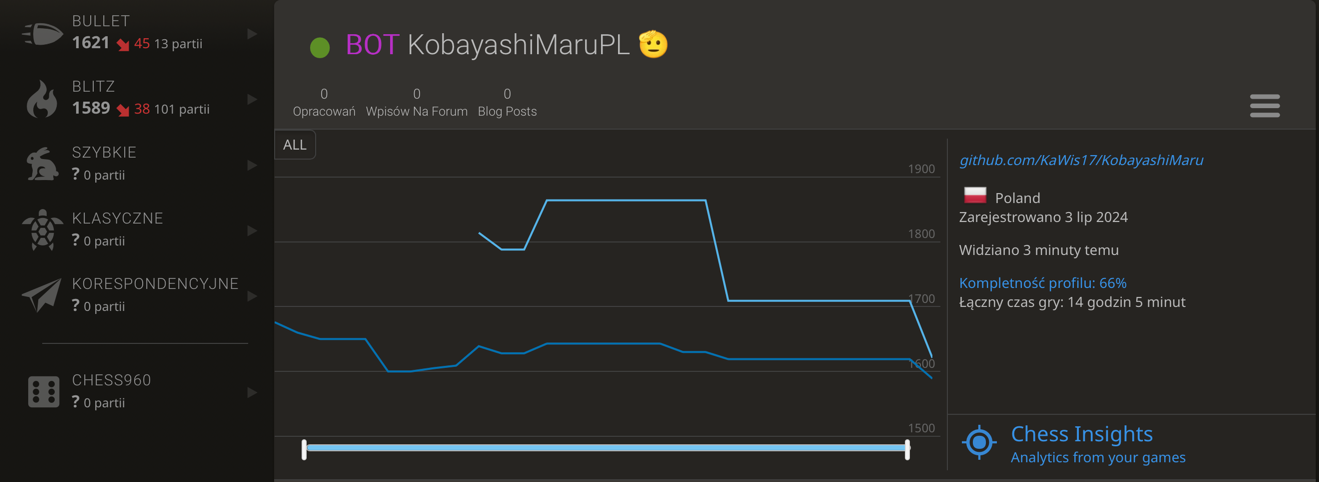
\includegraphics[width=1\linewidth]{rozdzialy/rozdzial03/2_porownanie-z-innymi-silnikami/rysunki/lichess-ranking}
    \caption{Ranking na platformie lichess}
    \label{fig:lichess-ranking}
\end{figure}
\section {Porównanie z graczami}
\label {sec: porownanie-z-graczami}

\subsection{Gra z autorem pracy}
\label{subsec:gra-z-autorem-pracy}

\subsection{Gra z graczem na poziomie 1800 ELO}
\label{subsec:gra-z-graczem-1800}

\subsection{Gra z krajowym mistrzem szachowym}
\label{subsec:gra-z-krajowym-mistrzem-szachowym}






\chapter{Zakończenie}
\label{ch:zakonczenie}

\section {Podsumowanie pracy}
\label {sec: podsumowanie-pracy}

\section {Możliwości dalszego rozwoju aplikacji}
\label {sec: dalszy-rozwoj}



% LITERATURA (zostanie wygenerowana automatycznie)
%UWAGA: bibliotekę referencji należy przygotować samemu. Dobrym do tego narzędziem jest JabRef.
%       JabRef oferuje jednak większą liczbę typów rekordów niż obsługuje BibTeX.
%       Proszę nie deklarować rekordów o typach nieobsługiwanych przez BibTeX.
%       Formatowania wykazu literatury i cytowań odbywać się ma zgodnie z zadeklarowanym stylem.
%       Zalecane są style produkujące numeryczne cytowania (w postaci [1], [2,3]).
%       Takim stylem jest np. plabbrv
\bibliographystyle{plabbrv}
%       Aby zapanować nad odstępami w wykazie literatury można posłużyć się poniższą komendą
\setlength{\bibitemsep}{2pt} % - zacieśnia wykaz
%       Pozycja Literatura pojawia się w spisie treści nieco inaczej niż spisy rysunków, tabel itp.
%       Aby zachować właściwe odstępy należy użyć poniższej komendy
\addtocontents{toc}{\addvspace{2pt}} % ustawiamy odstęp w spisie treści przed pozycją Literatura
%       Nazwę pliku przygotowanej biblioteki wpisuje się bez rozszerzenia .bib
%       (linia poniżej załaduje rekordy z pliku "dokumentacja.bib")
\printbibliography
\appendix
\chapter{Instrukcja wdrożenia}
\label{ch:instrukcja-wdrozenia}

\section{Rozgrywka na platformie Lichess}
\label{sec:rozgrywka-na-platformie-lichess}
Najłatwiejszym i najszybszym sposobem na zmierzenie się z silnikiem jest rozgrywka na platformie lichess.com, do czego autor niniejszej pracy serdecznie zaprasza.
Należy odszukać silnik po nazwie użytkownika \textit{KobayashiMaruPL} i gdy ten będzie aktywny zaprosić go~do~pojedynku.

W celu implementacji tego rozwiązania została wykorzystana biblioteka lichess-bot, która stanowi pośrednik pomiędzy silnikami wykorzystującymi UCI a API platformy Lichess. \cite{lichess-bot}

\section{Kompilacja kodu i połączenie z GUI}
\label{sec:kompilacja-kodu-i-polaczenie-z-gui}


\chapter{Protokół UCI}
\label{ch:protokol-uci}

\section{Wykorzystane komendy}
\label{sec:wykorzystane-komendy}

\begin{table}[htb] \small
\centering
\caption{UCI - komunikacja GUI do silnika}
\label{tab:UCI_GUI_silnik}
\begin{tabularx}{\linewidth}{|p{.35\linewidth}|X|}\hline
\textbf{Komenda} & \textbf{Opis działania} \\ \hline\hline

\texttt{uci} &
Określenie używanego protokołu.
Po otrzymaniu komendy silnik powinien odpowiedzieć \texttt{id} oraz listą dostępnych opcji.\\ \hline

\texttt{setoption name~<name> value~<value>} &
Instrukcja zmiany wewnętrznego parametru silnika.
Nazwa parametru jest podawana przez silnik.
Wartość może być typu bool, int, String. \\ \hline

\texttt{position [startpos~|~<fen>] moves <moves>} &
Ustawienie pozycji zaczynając od startowej bądź z~podanego FEN.
Możliwe wykonanie dalszych ruchów przekazanych w formacie LAN.\\ \hline

\texttt{isready} &
Zapytanie, służące synchronizacji GUI z silnikiem.
Gdy silnik nie przetwarza poleceń powinien odpowiedzieć \texttt{uciok}.\\ \hline

\texttt{go wtime~<wtime> btime~<btime> winc~<winc> binc~<binc>} &
Instrukcja rozpoczęcia szukania ruchu.
Kolejne argumenty w milisekundach wyrażają: pozostały czas białego i czarnego, dodatkowy czas per ruch białego i czarnego.\\ \hline

\texttt{debug [on | off]} &
Zmiana trybu diagnostycznego silnika. \\ \hline

\texttt{quit} &
Kończy działanie silnika. \\ \hline

\end{tabularx}
\end{table}

\begin{table}[htb] \small
\centering
\caption{UCI - komunikacja silnika do GUI}
\label{tab:UCI_silnik_GUI}
\begin{tabularx}{\linewidth}{|p{.35\linewidth}|X|}\hline
\textbf{Komenda} & \textbf{Opis działania} \\ \hline\hline

\texttt{id [name | author] <value>} &
Instrukcja służąca identyfikacji silnika przez GUI. \\ \hline

\texttt{option name <name> type <type>} &
Wypisanie dostępnych opcji oraz typu ich działania. \\ \hline

\texttt{uciok} &
Wysyłany po \texttt{id} oraz \texttt{option}, aby potwierdzić poprawne wykonanie komedny \texttt{uci}. \\ \hline

\texttt{readyok} &
Odpowiedź na \texttt{isready}.
Synchronizuje GUI z silnikiem.\\ \hline

\texttt{info <value>} &
Przekazywanie GUI informacji nad aktualnym stanem obliczeń najlepszego ruchu.\\ \hline

\texttt{bestmove <move>} &
Odpowiedź na instrukcję \texttt{go}.
Zwraca ruch proponowany przez silnik.\\ \hline

\end{tabularx}
\end{table}

\section{Przykład użycia}
\label{sec:przyklad-uzycia}

\begin{table}[htb] \footnotesize
\centering
\caption{Przykład użycia UCI}
\label{tab:przyklad_uci}
\begin{tabularx}{\linewidth}{|>{\raggedright\arraybackslash}p{.51\linewidth}>{\raggedleft\arraybackslash}X|}\hline
\textbf{Output GUI} & \textbf{Output silnika} \\ \hline\hline

\texttt{uci} & \texttt{} \\ \hline
\texttt{} & \texttt{
    id name KobayashiMaru \linebreak
    id author Krzysztof Antoni Wiśniewski \linebreak
    option name OwnBook type check \linebreak
    uciok
} \\ \hline
\texttt{setoption name OwnBook value false \linebreak
    isready
} & \texttt{} \\ \hline

\texttt{} & \texttt{readyok} \\ \hline
\texttt{position startpos \linebreak
    go wtime 60000 btime 60000 winc 600 binc 600} & \texttt{} \\ \hline
\texttt{} & \texttt{
    info depth 1 nodes 21 pv g1f3\linebreak
    info depth 2 nodes 177 pv d2d4 g8f6\linebreak
    ... \linebreak
    bestmove d2d4} \\ \hline

\texttt{position startpos moves d2d4 d7d5\linebreak
go wtime 58000 btime 55000 winc 600 binc 600} & \texttt{} \\ \hline

\texttt{...} & \texttt{...} \\ \hline
\texttt{quit} & \texttt{} \\ \hline

\end{tabularx}
\end{table}



%\include{dodatki.dodatekB}

% Jeśli w pracy pojawiać się ma indeks, należy odkomentować poniższe linie
%%\chapterstyle{noNumbered}
%%\phantomsection % sets an anchor
%%\addcontentsline{toc}{chapter}{Indeks rzeczowy}
%%\printindex

\end{document}
